\documentclass[a4paper,14pt]{extarticle}

\usepackage[T2A]{fontenc}			
\usepackage[utf8]{inputenc}			
\usepackage[english,russian]{babel}

\usepackage[
bookmarks=true, colorlinks=true, unicode=true,
urlcolor=black,linkcolor=black, anchorcolor=black,
citecolor=black, menucolor=black, filecolor=black,
]{hyperref}

\usepackage{color}
\usepackage{caption}
\DeclareCaptionFont{white}{\color{black}}
\DeclareCaptionFormat{listing}{\colorbox{white}{\parbox{\textwidth}{#1#2#3}}}
\captionsetup[lstlisting]{format=listing,labelfont=white,textfont=white}

\usepackage{amsmath,amsfonts,amssymb,amsthm,mathtools} 
\usepackage{wasysym}

\usepackage{graphicx}
%\usepackage[cache=false]{minted}
\usepackage{cmap}
\usepackage{indentfirst}

\usepackage{listings} 
\usepackage{fancyvrb}

\usepackage{geometry}
\geometry{left=2cm}
\geometry{right=1.5cm}
\geometry{top=1cm}
\geometry{bottom=2cm}

\setlength{\parindent}{5ex}
\setlength{\parskip}{0.5em}

\usepackage{color}
\usepackage[cache=false, newfloat]{minted}
\newenvironment{code}{\captionsetup{type=listing}}{}
\SetupFloatingEnvironment{listing}{name=Листинг}
 
 
 \begin{document}
 	
 	\def\figurename{Рисунок}
 	
 	\begin{minipage}{0.2\textwidth}
 		
\includegraphics[scale=0.05]{img/bmstu.png}
 	\end{minipage}
 	\begin{minipage}{0.7\textwidth}
 		\small
 		\begin{center}
 			\textbf{Министерство науки и высшего образования Российской Федерации}
 			
 			\textbf{Федеральное государственное бюджетное образовательное учреждение высшего образования «Московский государственный технический университет имени Н.Э. Баумана}
 			
 			\textbf{(национальный исследовательский университет)»}
 			
 			\textbf{(МГТУ им. Н.Э. Баумана)}
 		\end{center}
 	\end{minipage}
 	
 	\vspace*{5mm}
 	
 	\normalsize
 	\begin{flushleft}
 		Факультет: <<Информатика и системы управления>>
 		
 		Кафедра: <<Программное обеспечение ЭВМ и информационные технологии>>
 	\end{flushleft}
 	
 	\vspace*{30mm}
 	
 	\LARGE
 	\begin{center}
 		\textbf{Расчетно-пояснительная записка}
 		
 		%	\textbf{к курсовому проекту на тему:}
 		\textbf{к курсовой работе на тему:}
 		
 		\textbf{<<Web-приложение, содержащее информацию о вирусах>>}
 	\end{center}
 	
 	%\huge
 	%\begin{center}
 	%	\textbf{Лабораторная работа №9}
 	%\end{center}
 	%
 	%\begin{center}
 	%	\textbf{Тема:} <<Обработчики прерываний>>
 	%\end{center}
 	
 	\vspace*{15mm}
 	
 	\large
 	\begin{flushleft}
 		\textbf{Студент:} Левушкин И. К. \\
 		\textbf{Группа:} ИУ7-62Б \\
 		%        \textbf{Оценка (баллы):} \\
 		\textbf{Научный руководитель:} Гаврилова Ю.М.
 	\end{flushleft}
 	
 	\vspace*{50mm}
 	
 	\large
 	\begin{center}
 		Москва, 2020 г.
 	\end{center}
 	
 	\thispagestyle{empty}
 	
 	\newpage
 	
 	\section*{Задание на курсовой проект}
 	Разработать Web-приложение на языке программирования Python с использованием фреймворка Django. Основная задача данного приложения - хранение и показ информации о скорости распространения вируса, количестве зараженных, симптомов, вызываемых заболеванием, статистике выздоровевших и умерших от этого вируса в удобной для пользователя форме. Также, будет реализована возможность сравнивать графики (статистику) тех или вирусов. 
 	
 	В приложении можно будет осуществлять поиск вирусов по базе данных. Пользователь имеет возможность авторизоваться или зарегистрироваться в приложении, после этого пользователь сможет добавлять в избранное различную информацию про тот или иной вирус, что он просмотрел.
 	
 	
 	\newpage
 	
 	\tableofcontents
 	\newpage
 	\section*{Введение}
 	\addcontentsline{toc}{section}{Введение}
 	
 	Целью данной работы является закрепление навыков проектирования и создания реляционной базы данных, изучение особенностей разработки веб-интерфейса для работы с базой данных. Для выполнения поставленной задачи было спроектировано Web-приложение, в котором пользователи могут просматривать, редактировать и анализировать информацию о вирусах, регистрироваться и авторизоваться, добавлять в избранное понравивщуюся информацию. Это позволит исследовать  и изучить операции, которые присутствуют почти на многих современных проектах, а именно: чтение, редактирование и отображение информации из базы данных.
 	
 	Результатом выполнения данной работы является веб-сайт с  вышеописанным интерфейсом, а также замечания по поводу достоинств и недостатков тех или иных решений в разработке. Кроме того, будет приведена исследовательская информация по проекту, касающаяся работы базы данных.
 	
 	
 	\newpage
 	\section{Аналитический раздел}
 	
 	\subsection{Формализация задачи}\label{main}
 	
 	В соотвествии с техническим заданием необходимо разработать систему,
 	позволяющую осуществлять регистрацию учетной записи, вход в нее, выход из нее и ее редактирование.
 	
 	Неавторизованный пользователь может просматривать информацию о вирусах, эпидемиях и местах, где происходило распространение вируса.
 	
 	Авторизованный пользователь может добавлять понравившуюся информацию в избранное и анализировать ее. Анализ может осуществляться путем просмотра краткой информации о вирусе, а также построением графиков распространения вирусов.
 	
 	Также, программный комплекс будет предоставлять особые полномочия администраторам веб-приложения, а именно - редактирование информации о вирусах, эпидемиях и местах, где происходило распространение вируса.
 	
 	\subsection{Разбор различных СУБД}
 	
 	Несмотря на то, что все системы управления базами данных выполняют одну и ту же основную задачу (т.е. дают возможность пользователям создавать, редактировать и получать доступ к информации, хранящейся в базах данных), сам процесс выполнения этой задачи варьируется в широких пределах. Кроме того, функции и возможности каждой СУБД могут существенно отличаться. Различные СУБД документированы по-разному: более или менее тщательно. По-разному предоставляется и техническая поддержка. При сравнении различных популярных баз данных, следует учитывать, удобна ли для пользователя и масштабируема ли данная конкретная СУБД, а также убедиться, что она будет хорошо интегрироваться с другими продуктами, которые будут использоваться в системе. Для разработки была выбрана реляционная модель базы данных, поэтому рассмотрим три наиболее важные и популярные СУБД с открытым исходным кодом: SQLite\cite{sqlite}, MySQL\cite{mysql}, PostgreSQL\cite{postgresql}\cite{postgresql_better}.
 	
 	\subsubsection{SQLite}
 	
 	База данных SQLite накладывает минимальное количество ограничений на пользователя. База не предоставляет сетевого интерфейса и использует для своей работы единственный файл. Первоначально была разработана как облегченная версия MySQL без модулей, которые не используются во многих проектах. 
 	
 	Преимущества:
 	
 	\begin{itemize}
 		\item Главное преимущество заключается в том, что во встраиваемых или распределенных системах каждая машина несет полную реализацию базы данных. Это может значительно повысить производительность БД, поскольку снижает потребность в межпроцессных вызовах. Например, база встроена в ОС Android и предоставляет разработчикам приложений удобный интерфейс работы с ней.
 		\item База использует для работы единственный файл, что хорошо влияет на ее переносимость.
 		\item Система SQLite основана на языке запросов SQL, что удобно для разработки.
 		\item Подходит для небольших проектов с небольшими БД. 
 	\end{itemize}
 
 	Недостатки:
 	
 	\begin{itemize}
 		\item Отсутствие встроенного шифрования данных, что стало стандартом для предотвращения наиболее распространенных хакерских атак в интернете.
 		\item База не поддерживает систему учета пользователей, в то время как другие популярные СУБД поддерживают эту возможность.
 		\item Только одна операция записи за транзакцию, что уменьшает производительность системы
 	\end{itemize}
 
 	\subsubsection{MySQL}
 	
 	MySQL – самая популярная СУБД. Это многофункциональное открытое приложение, поддерживающее работу огромного количества сайтов. Система MySQL довольно проста в работе и может хранить большие массивы данных. Учитывая популярность MySQL, для этой системы было разработано большое количество сторонних приложений, инструментов и библиотек. MySQL не реализует полный стандарт SQL. Несмотря на это, MySQL предлагает множество функциональных возможностей для пользователей: автономный сервер баз данных, взаимодействие с приложениями и сайтами и т.п. 
 	
 	Преимущества:
 	
 	\begin{itemize}
 		\item Простота в работе: MySQL очень просто установить и настроить. Сторонние инструменты, в том числе визуализаторы (интерфейсы) значительно упрощают работу с данными.
 		\item Функциональность: MySQL поддерживает огромное количество функций SQL\cite{sql}.
 		\item Безопасность: MySQL предоставляет много встроенных продвинутых функций для защиты данных.
 		\item Масштабируемость и производительность: MySQL может работать с большими объёмами данных. 
 	\end{itemize}
 
 	Недостатки:
 	
 	\begin{itemize}
 		\item Ограничения: структура MySQL накладывает некоторые ограничения, из‒за которых не смогут работать продвинутые приложения.
 		\item Уязвимости: метод обработки данных, применяемый в MySQL, делает эту СУБД немного менее надёжной по сравнению с другими СУБД.
 		\item Медленное развитие: хотя MySQL является продуктом с открытым исходным кодом, он очень медленно развивается. Однако тут следует заметить, что на MySQL основано несколько полноценных баз данных (например, MariaDB).
 	\end{itemize}
 
 	\subsubsection{PostgreSQL}
 	
 	PostgreSQL – это продвинутая открытая объектно‒ориентированная СУБД. Часто используется при разработке веб-сайтов. Позволяет разработчикам управлять как структурированными, так и неструктурированными данными. Может быть использована на большинстве основных платформ, включая Linux и MacOS. В отличие от других СУБД, PostgreSQL поддерживает очень важные объектно‒ориентированные и реляционные функции баз данных: надежные транзакции ACID (атомарность, согласованность, изолированность, долговечность) и т.п. СУБД PostgreSQL основана на надежной технологии, она может одновременно обрабатывать большое количество задач. Хотя СУБД PostgreSQL не так популярна, как MySQL, для неё тоже разработано большое количество дополнительных инструментов и библиотек, которые упрощают работу с данными и увеличивают производительность СУБД.
 	
 	Преимущества:
 	
 	\begin{itemize}
 		\item PostgreSQL имеет открытый исходный код.
 		\item База использует язык запросов SQL.
 		\item PostgreSQL обладает большим сообществом разработчиков, которые помогут найти решение любой проблемы, связанной с СУБД, в любое время суток.
 		\item Помимо встроенных функций, PostgreSQL поддерживает множество открытых сторонних инструментов для проектирования, управления данными и т.п. Одним из таких инструментов является веб-приложение pgAdmin.
 		\item База очень хорошо масштабируется и расширяется.
 		\item Работает быстро и надежно, база способна обрабатывать терабайты данных.
 		\item Поддерживает формат json.
 	\end{itemize}
 
 	Недостатки:
 	
 	\begin{itemize}
 		\item Производительность в некоторых ситуациях ниже, чем у MySQL.
 		\item Невысокая популярность, однако все больше проектов используют PostgreSQL в качестве СУБД.
 	\end{itemize}
 
 	\subsection{Django}
 	
 	Django\cite{django} — фреймворк для веб‒приложений на языке Python\cite{python}. Один из основных принципов фреймворка — DRY (don't repeat yourself). Веб‒системы на Django строятся из одного или нескольких приложений, которые рекомендуется делать отчуждаемыми и подключаемыми. Это одно из заметных архитектурных отличий этого фреймворка от некоторых других, например, Ruby on Rails. Также, в отличие от многих других фреймворков, обработчики URL в Django конфигурируются явно при помощи регулярных выражений, а не автоматически задаются из структуры контроллеров.
 	
 	Django проектировался для работы под управлением Apache с модулем mod\_python и с использованием PostgreSQL в качестве базы данных. В настоящее время, помимо PostgreSQL, Django может работать с другими СУБД: MySQL, SQLite, Microsoft SQL Server, DB2, Firebird, SQL Anywhere 9 и Oracle. Для работы с базой данных Django использует собственный ORM, в котором модель данных описывается классами Python, и по ней генерируется схема базы данных.
 	
 	Архитектура Django похожа на MVC\cite{mvc_info} (Model‒View–Controller). Контроллер классической модели MVC примерно соответствует уровню, который в Django называется Представлением (View), а презентационная логика Представления реализуется в Django уровнем Шаблонов (Templates). Из‒за этого уровневую архитектуру Django часто называют MTV (Model-Template-View).
 	
 	Первоначально разработка Django велась для обеспечения более удобной работы с новостными ресурсами, что достаточно сильно отразилось на архитектуре: фреймворк предоставляет ряд средств, которые помогают в быстрой разработке веб‒сайтов информационного характера. Например, разработчику не требуется создавать контроллеры и страницы для административной части сайта, в Django есть встроенное приложение для управления содержимым, которое можно включить в любой сайт, сделанный на Django, и которое может управлять сразу несколькими сайтами на одном сервере. Административное приложение позволяет создавать, изменять и удалять любые объекты наполнения сайта, протоколируя все совершённые действия, и предоставляет интерфейс для управления пользователями и группами.
 	
 	Веб‒фреймворк Django используется в таких крупных и известных сайтах, как Instagram, Disqus, Mozilla, The Washington Times, Pinterest, lamoda. 
 	
 	Преимущества:
 	
 	\begin{itemize}
 		\item Простота в изучении.
 		\item Чистота и читаемость.
 		\item Разносторонность.
 		\item Быстрота написания.
 		\item Цельный дизайн
 	\end{itemize}
 
 	\subsection*{Выводы по аналитическому разделу}
 	
 	Исходя из представленной выше информации было принято решение использовать СУБД PostgreSQL, поскольку она обладает множеством открытых сторонних инструментов проектирования и управления данными, такими как pgAdmin, которые значительно упрощают разработку базы данных. Также, при своем проектировании фреймворк Django, используемый в данной работе, использовал PostgreSQL в качестве базы данных. Поэтому чтобы избежать непредвиденных трудностей при разработке ПО былор решено использовать PostgreSQL.
 	
 	\newpage
 	\section{Конструкторский раздел}
 	
 	\subsection{USE-CASE диаграмма}
 	
 	Формулировка требования к возможностям программного обеспечения из раздела \ref{main} требует большей конкретики.
 	Диаграмма вариантов использования (рисунок \ref{ris:use}) описывает взаимоотношения и зависимости между группами вариантов использования и действующими лицами, участвующими в процессе.
 	
 	\begin{figure}[h!]
 		\begin{center}
 			{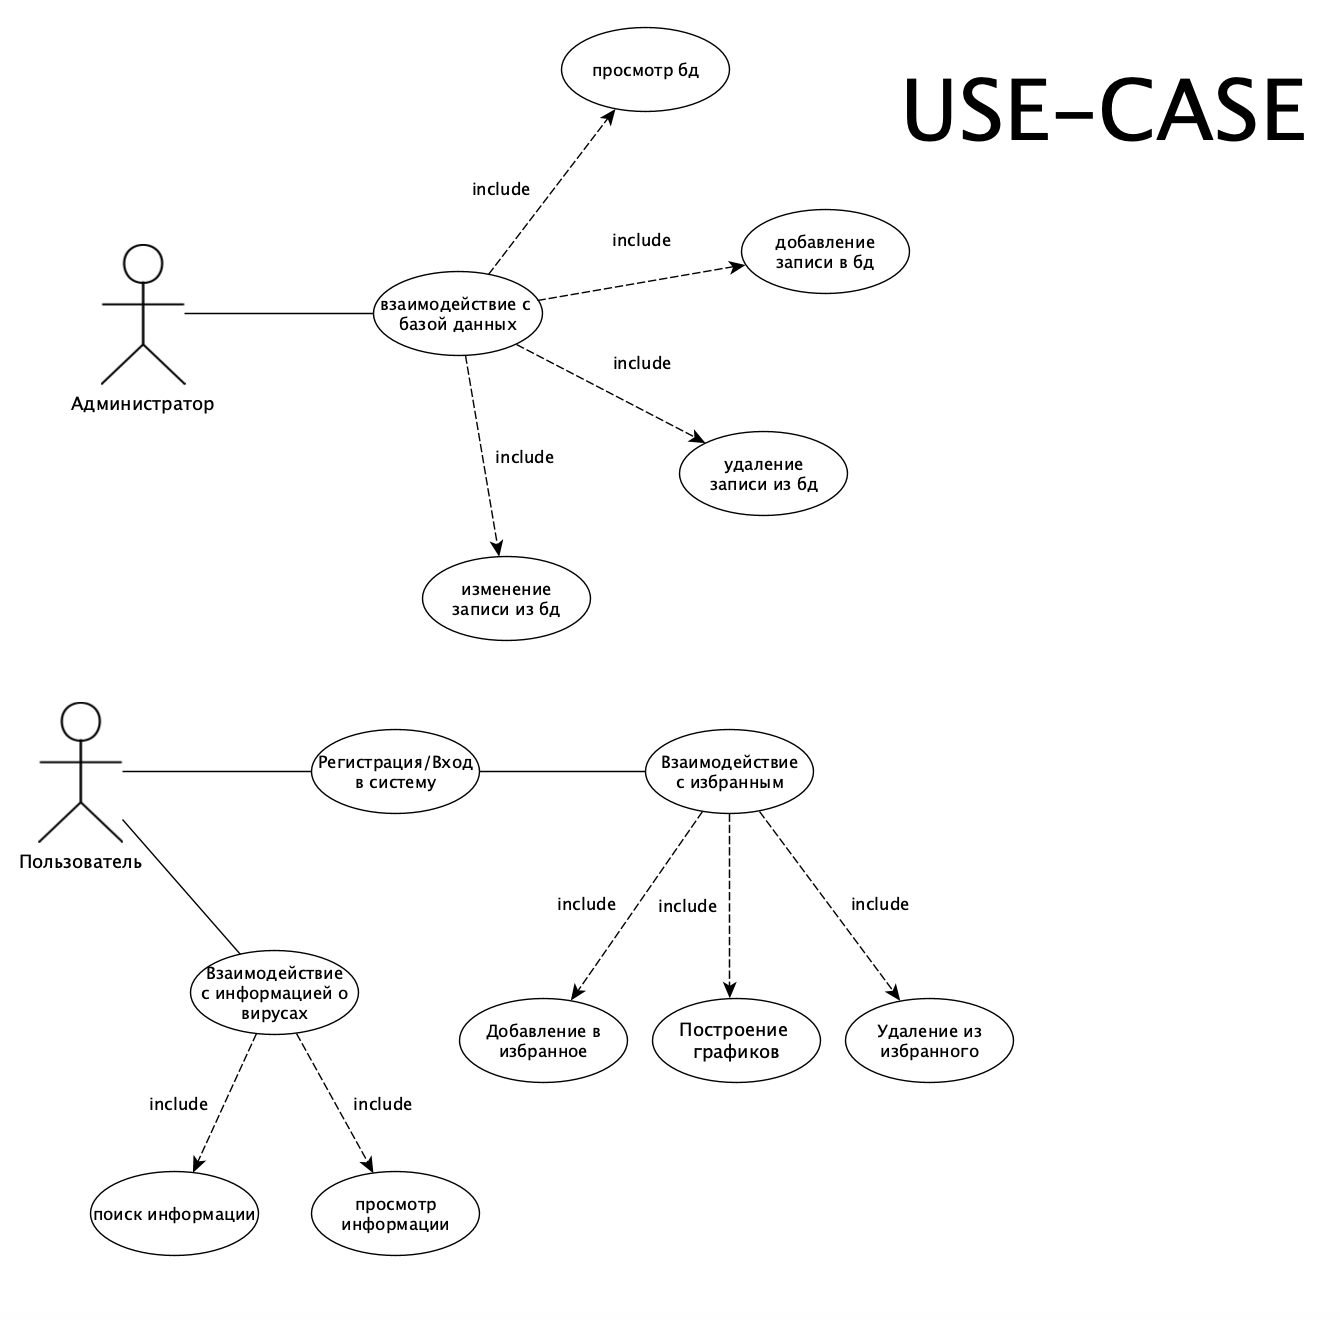
\includegraphics[width = 0.8\textwidth]{diagram/USE-CASE.png}}
 			\caption{
 				USE-CASE диаграмма}
 			\label{ris:use}
 		\end{center}
 	\end{figure}

 	
 	Важно понимать, что диаграммы вариантов использования не предназначены для отображения проекта и не могут описывать внутреннее устройство системы. Диаграммы прецедентов предназначены для упрощения взаимодействия с будущими пользователями системы, с клиентами, и особенно пригодятся для определения необходимых характеристик системы. Другими словами, диаграммы вариантов использования говорят о том, что система должна делать, не указывая сами применяемые методы \cite{usecase}.
 	
 	\subsection{Структура базы данных}
 	
 	\subsubsection{ER-диаграмма}
 	
 	С помощью диаграммы «сущность — связь» (рисунок \ref{ris:er}) описывается концептуальная схема предметной области \cite{er}.
 	Графическое отображение дает четкое представление о действующих сущностях и их атрибутах, а также устанавливает связи между различными сущностями.
 	
 	\begin{figure}[h!]
 		\begin{center}
 			{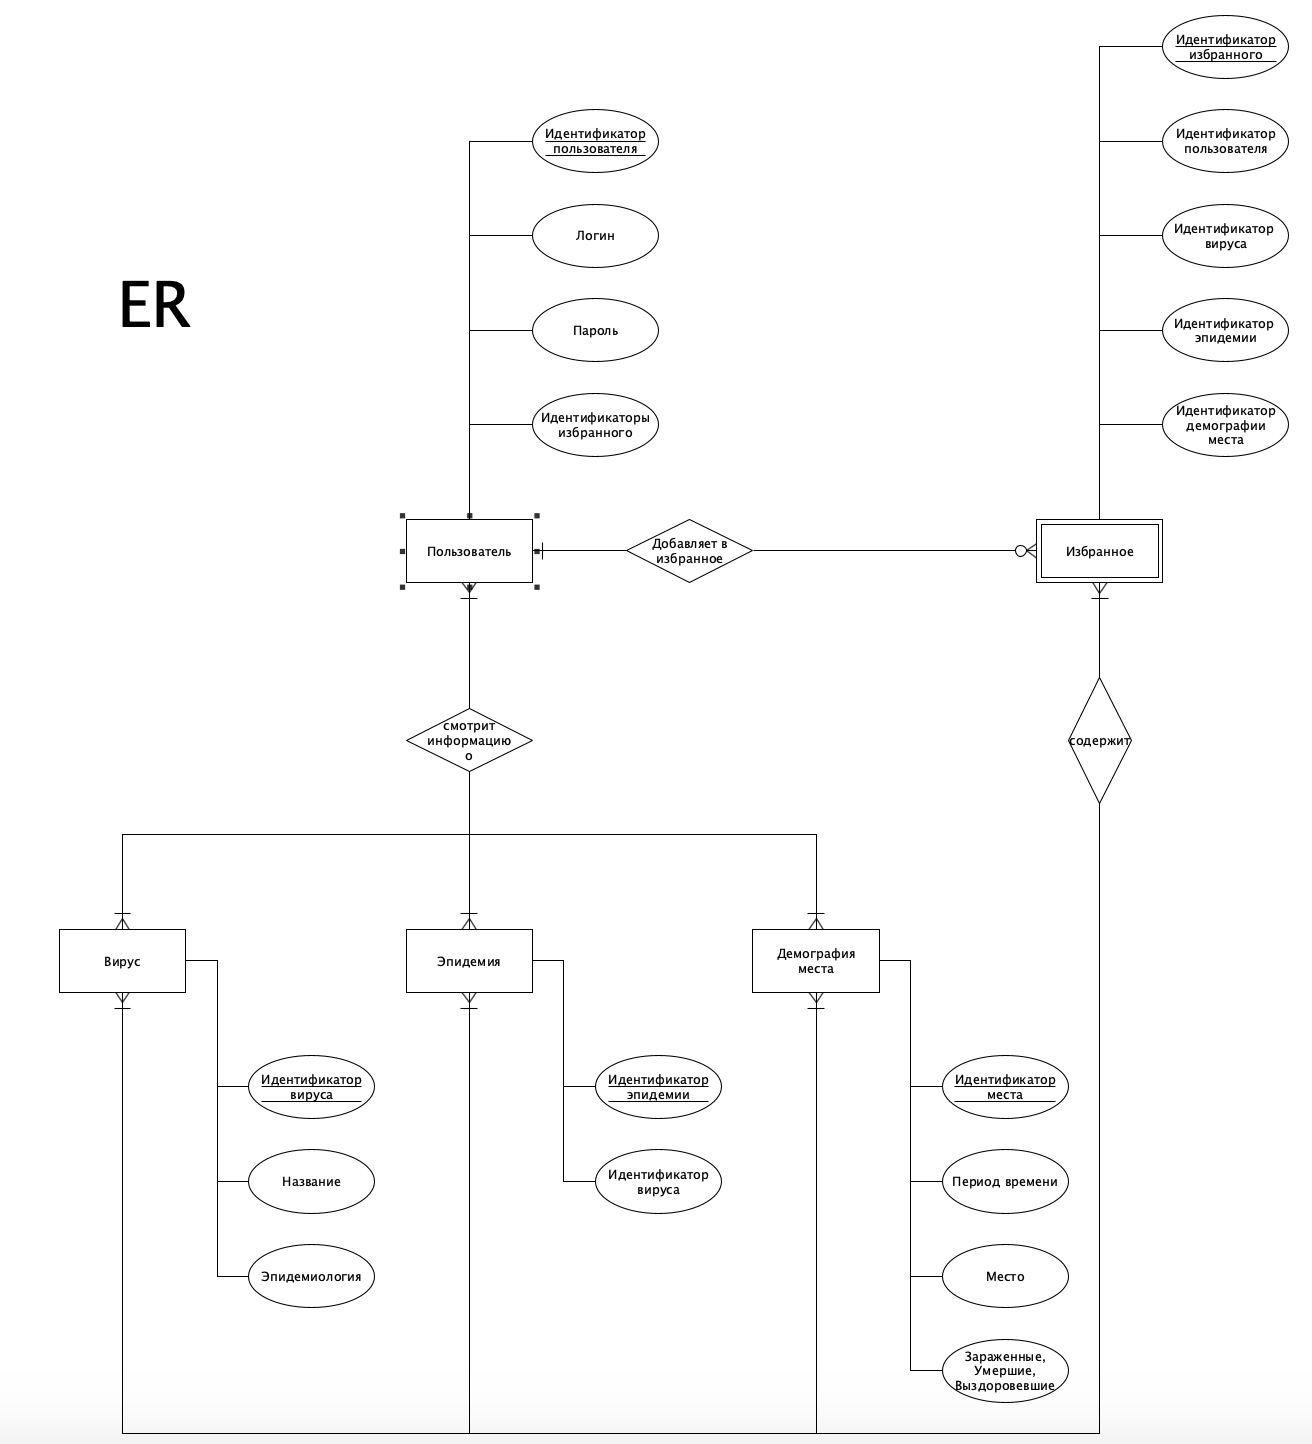
\includegraphics[width = \textwidth]{diagram/ER.png}}
 			\caption{
 				Диаграмма «сущность — связь»}
 			\label{ris:er}
 		\end{center}
 	\end{figure}
 	
 	\subsubsection{Диаграмма базы данных}
 	
 	Ниже приведена диаграмма базы данных, показывающая виды связей между таблицами и основной набор их атрибутов.
 	
 	\begin{figure}[h!]
 		\begin{center}
 			{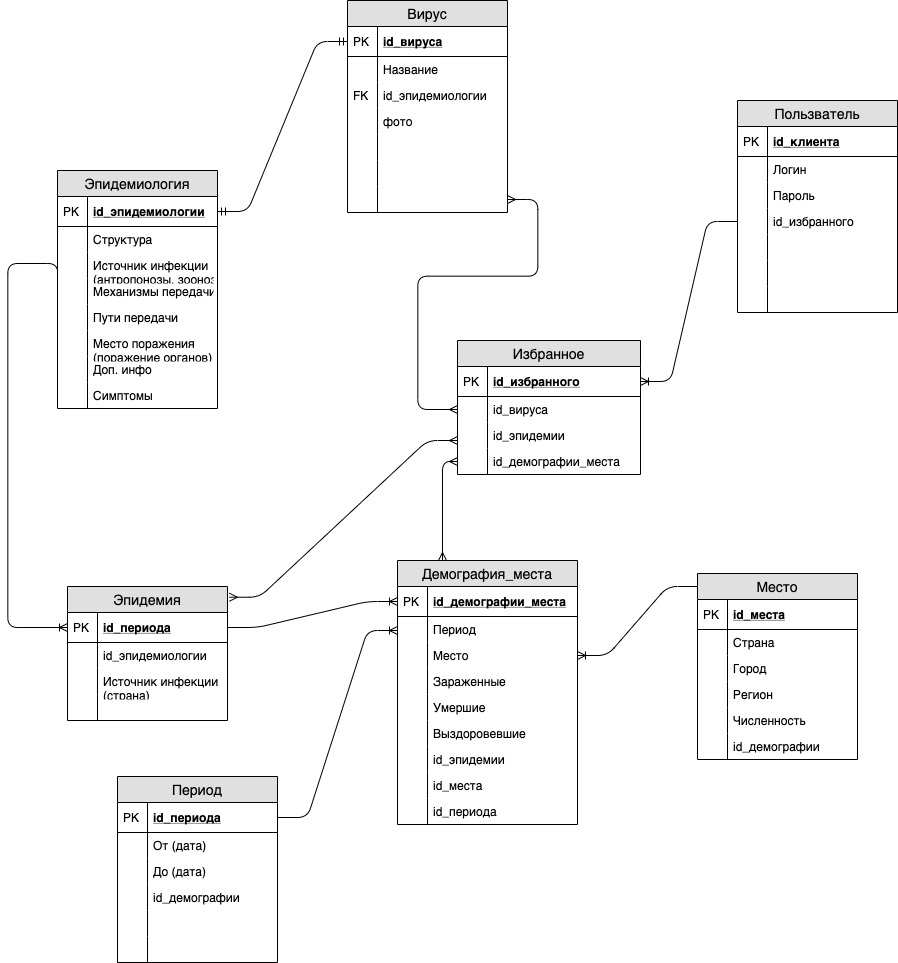
\includegraphics[width = \textwidth]{diagram/bd_diagram.png}}
 			\caption{
 				Диаграмма «сущность — связь»}
 			\label{ris:bd}
 		\end{center}
 	\end{figure}
 
 	\newpage
 	
 	\subsubsection{UML диаграмма данных}
 	
 	Ниже приведена UML схема ассоциаций между таблицами базы данных и их взаимосвязь.
 	
 	\begin{figure}[h!]
 		\begin{center}
 			{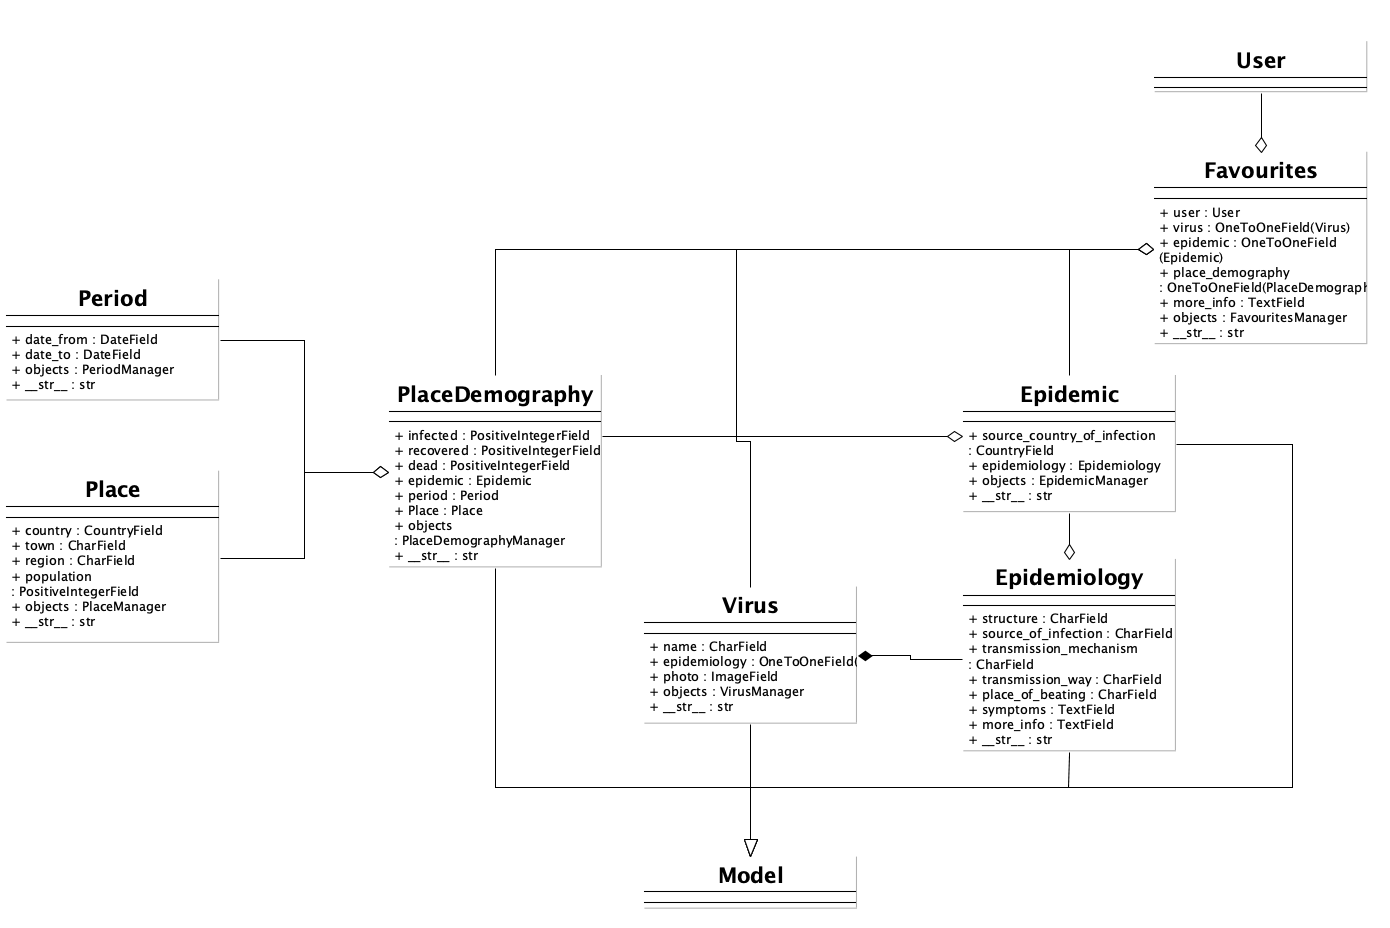
\includegraphics[width = \textwidth]{diagram/data_uml.png}}
 			\caption{
 				Диаграмма «сущность — связь»}
 			\label{ris:data_uml}
 		\end{center}
 	\end{figure}
 
 	\newpage
 
 	\subsection{Менеджеры приложения}
 	
 	В приложении реализованы менеджеры, которые позволяют управлять записями базы данных.
 	
 	Ниже приведена UML схема менеджеров приложения.
 	
 	\begin{figure}[h!]
 		\begin{center}
 			{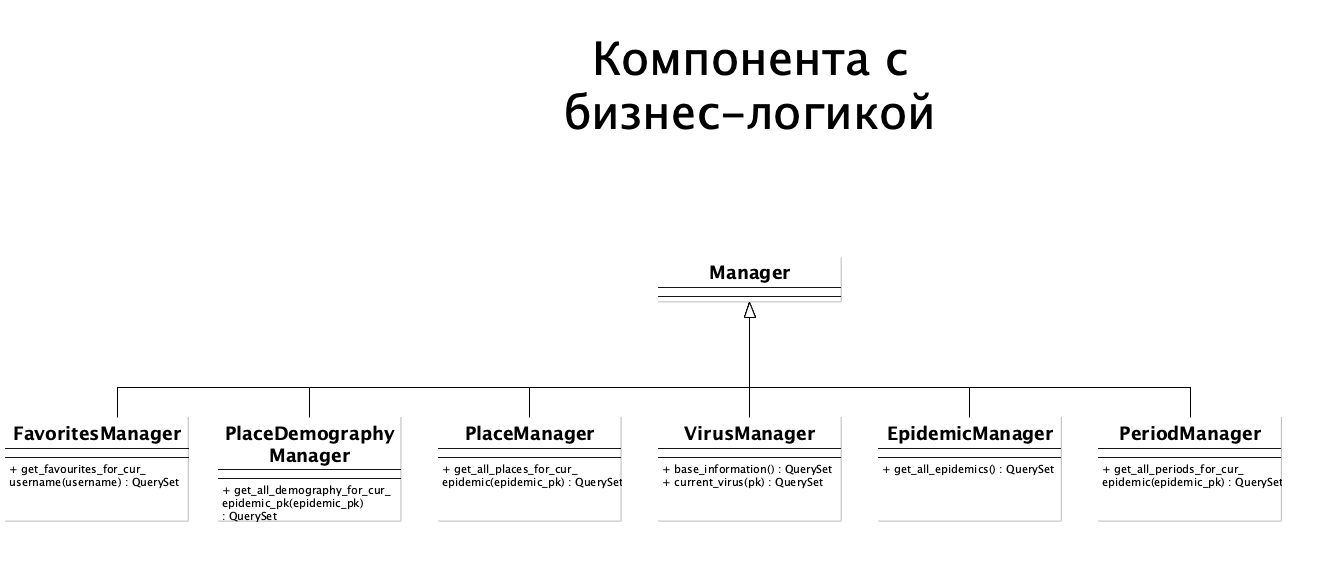
\includegraphics[width = \textwidth]{diagram/managers.png}}
 			\caption{
 				Диаграмма «сущность — связь»}
 			\label{ris:managersl}
 		\end{center}
 	\end{figure}
 	
 	Где
 	\begin{itemize}
 		\item VirusManager имеет 2 метода:
 		\begin{itemize}
 			\item base\_information(self) - сортирует все вирусы по их названию;
 			\item current\_virus(self, pk) - получает вирус по его id;
 		\end{itemize}
 		\item EpidemicManager имеет 4 метода:
 		\begin{itemize}
 			\item current\_epidemic(self, pk) - получает эпидемию по ее id;
 			\item get\_all\_epidemics(self) - сортирует все эпидемии по названию страны-источника заражения;
 			\item get\_epidemics\_by\_epidemiology\_pk(self, epidemiology\_pk) - получает все эпидемии по id эпидемиологии и преобразует их к удобной форме вывода на экран;
 			\item post\_changes\_in\_epidemic(self, pk, request) - получает эпидемию по ее id и применяет к ней изменения из запроса request;
 		\end{itemize}
 		\item PlaceDemographyManager имеет 7 методов:
 		\begin{itemize}
 			\item get\_places\_demography\_by\_epidemic\_pk(self, epidemic\_pk) - получает все демографии места по id эпидемии;
 			\item get\_regions\_by\_epidemic\_pk(self, epidemic\_pk),
 			
 			 get\_countries\_by\_region\_pk(self, epidemic\_id, region\_name),
 			 
 			  get\_towns\_by\_country\_pk(self, epidemic\_id, region\_name, country\_name) - функции выполняют сложные sql-запросы (с применением group by), чтобы получить сжатую информацию о регионах, странах и городах, соответственно;
 			\item get\_current\_region\_sql(self, epidemic\_pk, region\_name),
 			
 			 get\_current\_country\_sql(self, epidemic\_pk, region\_name, country\_name),
 			 
 			  get\_current\_town\_sql(self, epidemic\_pk, region\_name, country\_name, town\_name) - функции выполняют sql-запросы и получают информацию о конкретном регионе, стране, городе, соответственно;
 		\end{itemize}
 		\item PeriodManager имеет 1 метод:
 		\begin{itemize}
 			\item get\_all\_periods\_for\_cur\_epidemic(self, epidemic\_pk) - получает все периоды времени по id эпидемии и сортирует их по дате;
 		\end{itemize}
 		\item PlaceManager имеет 1 метод:
 		\begin{itemize}
 			\item get\_all\_places\_for\_cur\_epidemic(self, epidemic\_pk) - получает все места заражения по id эпидемии;
 		\end{itemize}
 		\item FavouritesManager имеет 17 методов:
 		\begin{itemize}
 			\item get\_all\_viruses\_by\_username(self, username),
 			
 			 get\_all\_epidemics\_by\_username(self, username),
 			 
 			  get\_all\_regions\_by\_username(self, username),
 			  
 			   get\_all\_countries\_by\_username(self, username),
 			   
 			    get\_all\_towns\_by\_username(self, username)  - возвращает все добавленные конкретным пользователем вирусы, эпидемии, регионы, страны, города, соответственно, в избранное;
 			\item - add\_region(self, epidemic\_pk, region\_name, user), 
 			
 			add\_country(self, epidemic\_pk, region\_name, country\_name, user),
 			
 			 add\_town(self, epidemic\_pk, region\_name, country\_name, town\_name, user) - добавляет регион, страну, город, соответственно, в избранное к конкретному пользователю;
 			\item delete\_region(self, epidemic\_pk, region\_name, username),
 			
 			 delete\_country(self, epidemic\_pk, region\_name, country\_name, username),
 			 
 			  delete\_town(self, epidemic\_pk, region\_name, country\_name, town\_name, username) - удаляет регион, страну, город из избранного конкретного пользователя;
 			\item get\_region\_graphics\_data(self, regions\_info),
 			
 			 get\_country\_graphics\_data(self, countries\_info),
 			 
 			  get\_town\_graphics\_data(self, towns\_info) - получает информацию о регионах, странах, городах, соответственно, в формате, используемым в дальнейшем для рисования графиков;
 		\end{itemize}
 	\end{itemize}
 	
 	\subsection*{Выводы по конструкторскому разделу}
 	
 	В данном разделе была приведена диаграмма вариантов использования, описана стуктура базы данных при помощи ER-диаграммы, диаграммы базы данных и UML диаграммы данных. Также были выделены менеджеры приложения, через которые будут осуществляться запросы к базе данных.
 	
 	\newpage
 	\section{Технологический раздел}
 	
 	\subsection{Технологический стек}
 	
 	\textit{\bf Front-end:}
 	\begin{itemize}
 		\item Язык гипертекстовой разметки HTML5\cite{html}
 		\item Таблицы стилей CSS3\cite{css} + Bootstrap4\cite{bootstrap}
 		\item Язык программирования JavaScript\cite{js}
 	\end{itemize}
 	
 	\textit{\bf Back-end:}
 	\begin{itemize}
 		\item СУБД PostgreSQL\cite{postgresql}
 		\item Фреймворк Django\cite{django}
 		\item Язык программирования Python3\cite{python}
 		\item Библиотеки:
 		\begin{itemize}
 			\item psycopg2\cite{psycopg2} - библиотека python для связи с PostgreSQL
 			\item django-countries~\cite{countries} - список всех стран мира
 		\end{itemize}
 	\end{itemize}
 
 	\newpage
 
 	\subsection{Реализация хранения данных}
 	
 	В листингах \ref{code:virus}-\ref{code:profile} сообщается о представлении
 	сущностей в Django. Выделенные классы соответствуют схеме базы данных из предыдущего раздела (рисунок ~\ref{ris:bd}).
 	
 	\begin{code}
 	\captionof{listing}{Представление модели <<вирус>>}
 	\label{code:virus}
 	\inputminted
 	[
 	frame=single,
 	framesep=10pt,
 	fontsize=\normalsize,
 	%linenos,
 	numbersep=5pt,
 	]
 	{python}
 	{code/virus.py}
 	\end{code}
 
 	\begin{code}
 		\captionof{listing}{Представление модели <<эпидемия>>}
 		\label{code:epidemic}
 		\inputminted
 		[
 		frame=single,
 		framesep=10pt,
 		fontsize=\normalsize,
 		%linenos,
 		numbersep=5pt,
 		]
 		{python}
 		{code/epidemic.py}
 	\end{code}

 
 	\begin{code}
 		\captionof{listing}{Представление модели <<профиль>>}
 		\label{code:profile}
 		\inputminted
 		[
 		frame=single,
 		framesep=10pt,
 		fontsize=\normalsize,
 		%linenos,
 		numbersep=5pt,
 		]
 		{python}
 		{code/profile.py}
 	\end{code}
 	
 
 	\newpage
 	
 	\subsection{URL-адреса}
 	
 	В Django используется так называемый URLconf (URL configuration). URLconf — это набор шаблонов, которые Django попробует сравнить с полученным URL, чтобы выбрать правильный метод для представления (view). Django сопоставляет URL–адреса, используя регулярные выражения (regular expressions). Регулярные выражения имеют множество правил, которые формируют поисковый шаблон. Ниже будет представлен список URL-шаблонов в проекте.
 	
 	
 	\begin{code}
 		\captionof{listing}{url-шаблоны}
 		\label{code:urls}
 		\inputminted
 		[
 		frame=single,
 		framesep=10pt,
 		fontsize=\normalsize,
 		%linenos,
 		numbersep=5pt,
 		]
 		{python}
 		{code/urls.py}
 	\end{code}
 	
 	\newpage
 	
 	\subsection{View}
 	
 	View или представление — это то место, где размещается логика работы приложения. Оно запрашивает информацию о модели, которую мы создали ранее и передаст её в шаблон и после этого приложение берет из базы данных значения, необходимые для отображения на странице. Ниже будет представлен пример View в проекте - virus.py.
 	
 	\begin{code}
 		\captionof{listing}{virus.py}
 		\label{code:view_virus}
 		\inputminted
 		[
 		frame=single,
 		framesep=10pt,
 		fontsize=\normalsize,
 		%linenos,
 		numbersep=5pt,
 		]
 		{python}
 		{code/view_virus.py}
 	\end{code}
 	
 	\newpage
 	
 	\subsection{HTML}
 	
 	HTML — это код, который может быть интерпретирован браузером, таким как Chrome, Firefox или Opera, чтобы отобразить веб–страницу пользователю. HTML (HyperText Markup Language) — язык гипертекстовой разметки. Гипертекст — это тип текста, поддерживающий гиперссылки между страницами. Под разметкой понимается введение в текст документа кода, который будет говорить браузеру, как интерпретировать веб‒страницу. HTML код строится при помощи тегов, каждый из которых должен начинаться с < и заканчиваться >. Эти теги представляют элементы разметки. Ниже будет приведен пример HTML файла проекта - profile.html.
 	
 	
 	\begin{code}
 		\captionof{listing}{profile.html}
 		\label{code:template_profile}
 		\inputminted
 		[
 		frame=single,
 		framesep=10pt,
 		fontsize=\normalsize,
 		%linenos,
 		numbersep=5pt,
 		]
 		{html}
 		{code/profile.html}
 	\end{code}
 
 	\newpage
 	
 	\subsection{Заполнение базы данных}
 	
 	Первое, о чем стоит задуматься при создании базы данных – это ее наполнение. В проекте достаточно большое количество таблиц и сущностей, поэтому задача ее наполнения – важнейший аспект работы. Был написан скрипт на языке Python, который генерирует необходимую информацию, используя за основу логистическое уравнение\cite{formula}, которое хорошо описывает скорость размножения популяции:
 	
 	\[
 	\frac{K P_0 e^{rt}}{K + P_0 (e^{rt} - 1)}
 	\]
 	
 	Где
 	\begin{itemize}
 		\item K - отвечает за растяжение графика вдоль оси y
 		\item P\_0 - отвечает за смещение смысловой части графика вдоль оси x
 		\item r - отвечает за растяжение смысловой части графика вдоль оси x
 	\end{itemize}
 	
 	Варьируя различные параметры формулы с помощью модуля random из стандартной библиотеки python, и происходила генерация данных. Далее эти данные записывались в файлы csv формата, откуда позже с помощью еще одного написанного скрипта на языке Python, преобразовывались в формат json и загружались в базу данных командой:
 	
 	\textit{python3 manage.py loaddata myapp/data/current\_data.json}
 	
 	\newpage
 	
 	\subsection{Примеры работы программы}
 	
 	Ниже будут приведены различные примеры работы программы и комментарии к ним.
 	
 	\begin{figure}[h!]
 		\begin{center}
 			{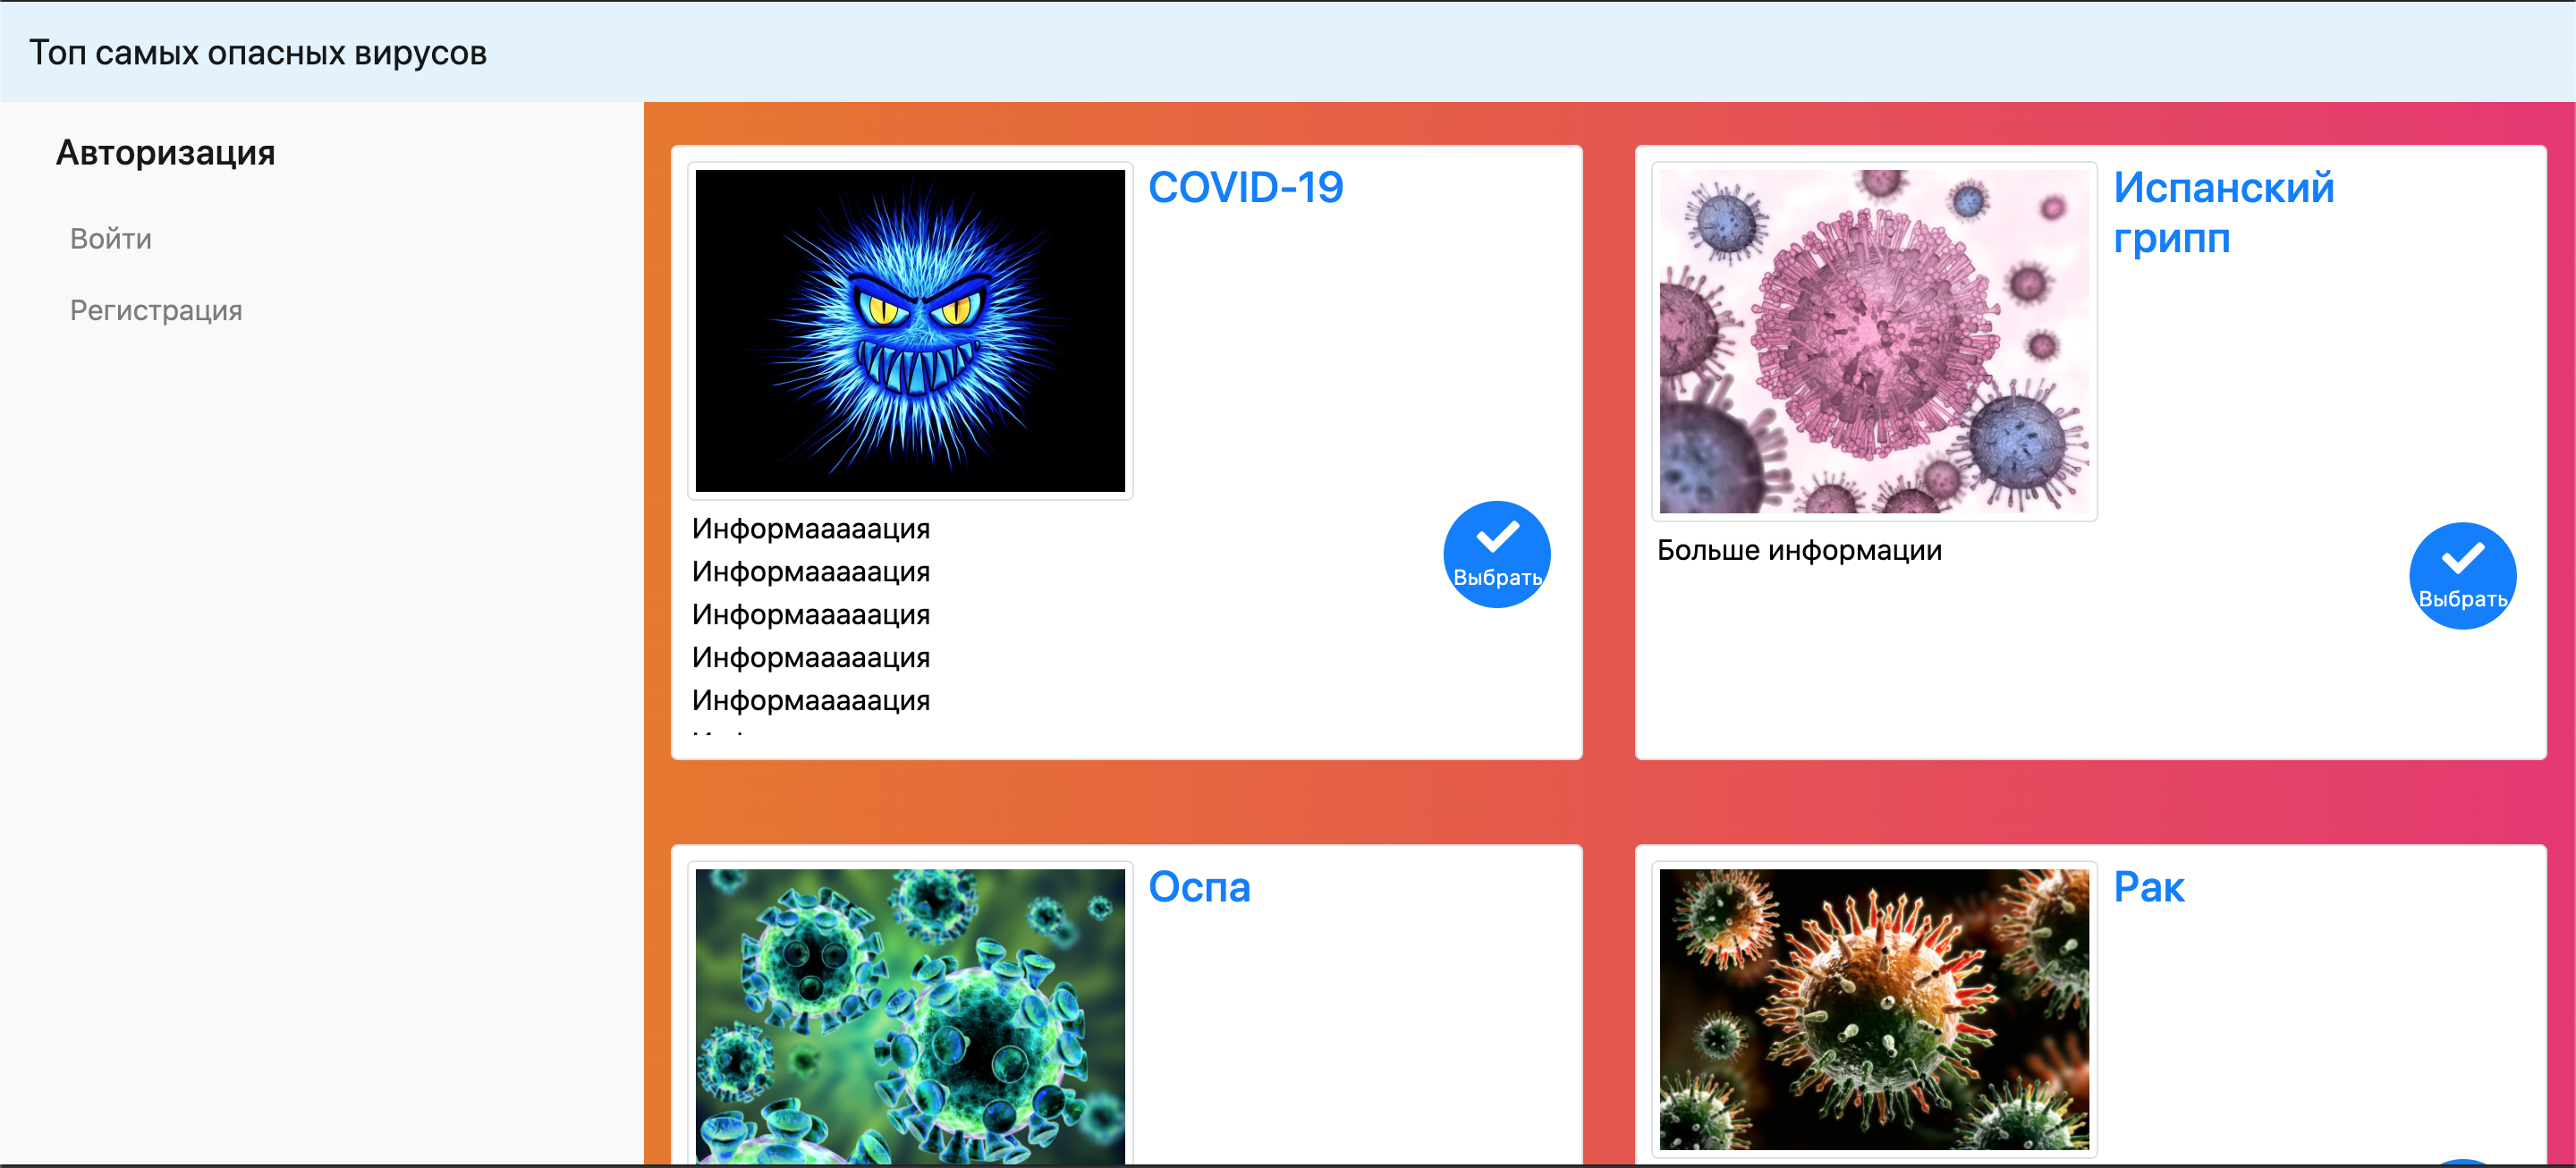
\includegraphics[width = \textwidth]{examples/main.png}}
 			\caption{
 				Главная страница (список вирусов)}
 			\label{ris:main}
 		\end{center}
 	\end{figure}
 	
 	На главной странице сайта можно увидеть список вирусов с краткой информацией о них. Далее можно спуститься на уровень ниже, нажав на кнопку "выбрать", и получить список всех эпидемий, связанных с этим вирусом. Аналогично, нажав на кнопку "выбрать", можно спуститься еще на уровень ниже и получить список всех регионов, в которых этот вирус распространялся, затем всех стран, находящихся в этом регионе, всех городов, относящихся к данной стране.
 	
 	\newpage
 	
 	\begin{figure}[h!]
 		\begin{minipage}[b]{0.45\textwidth}
 			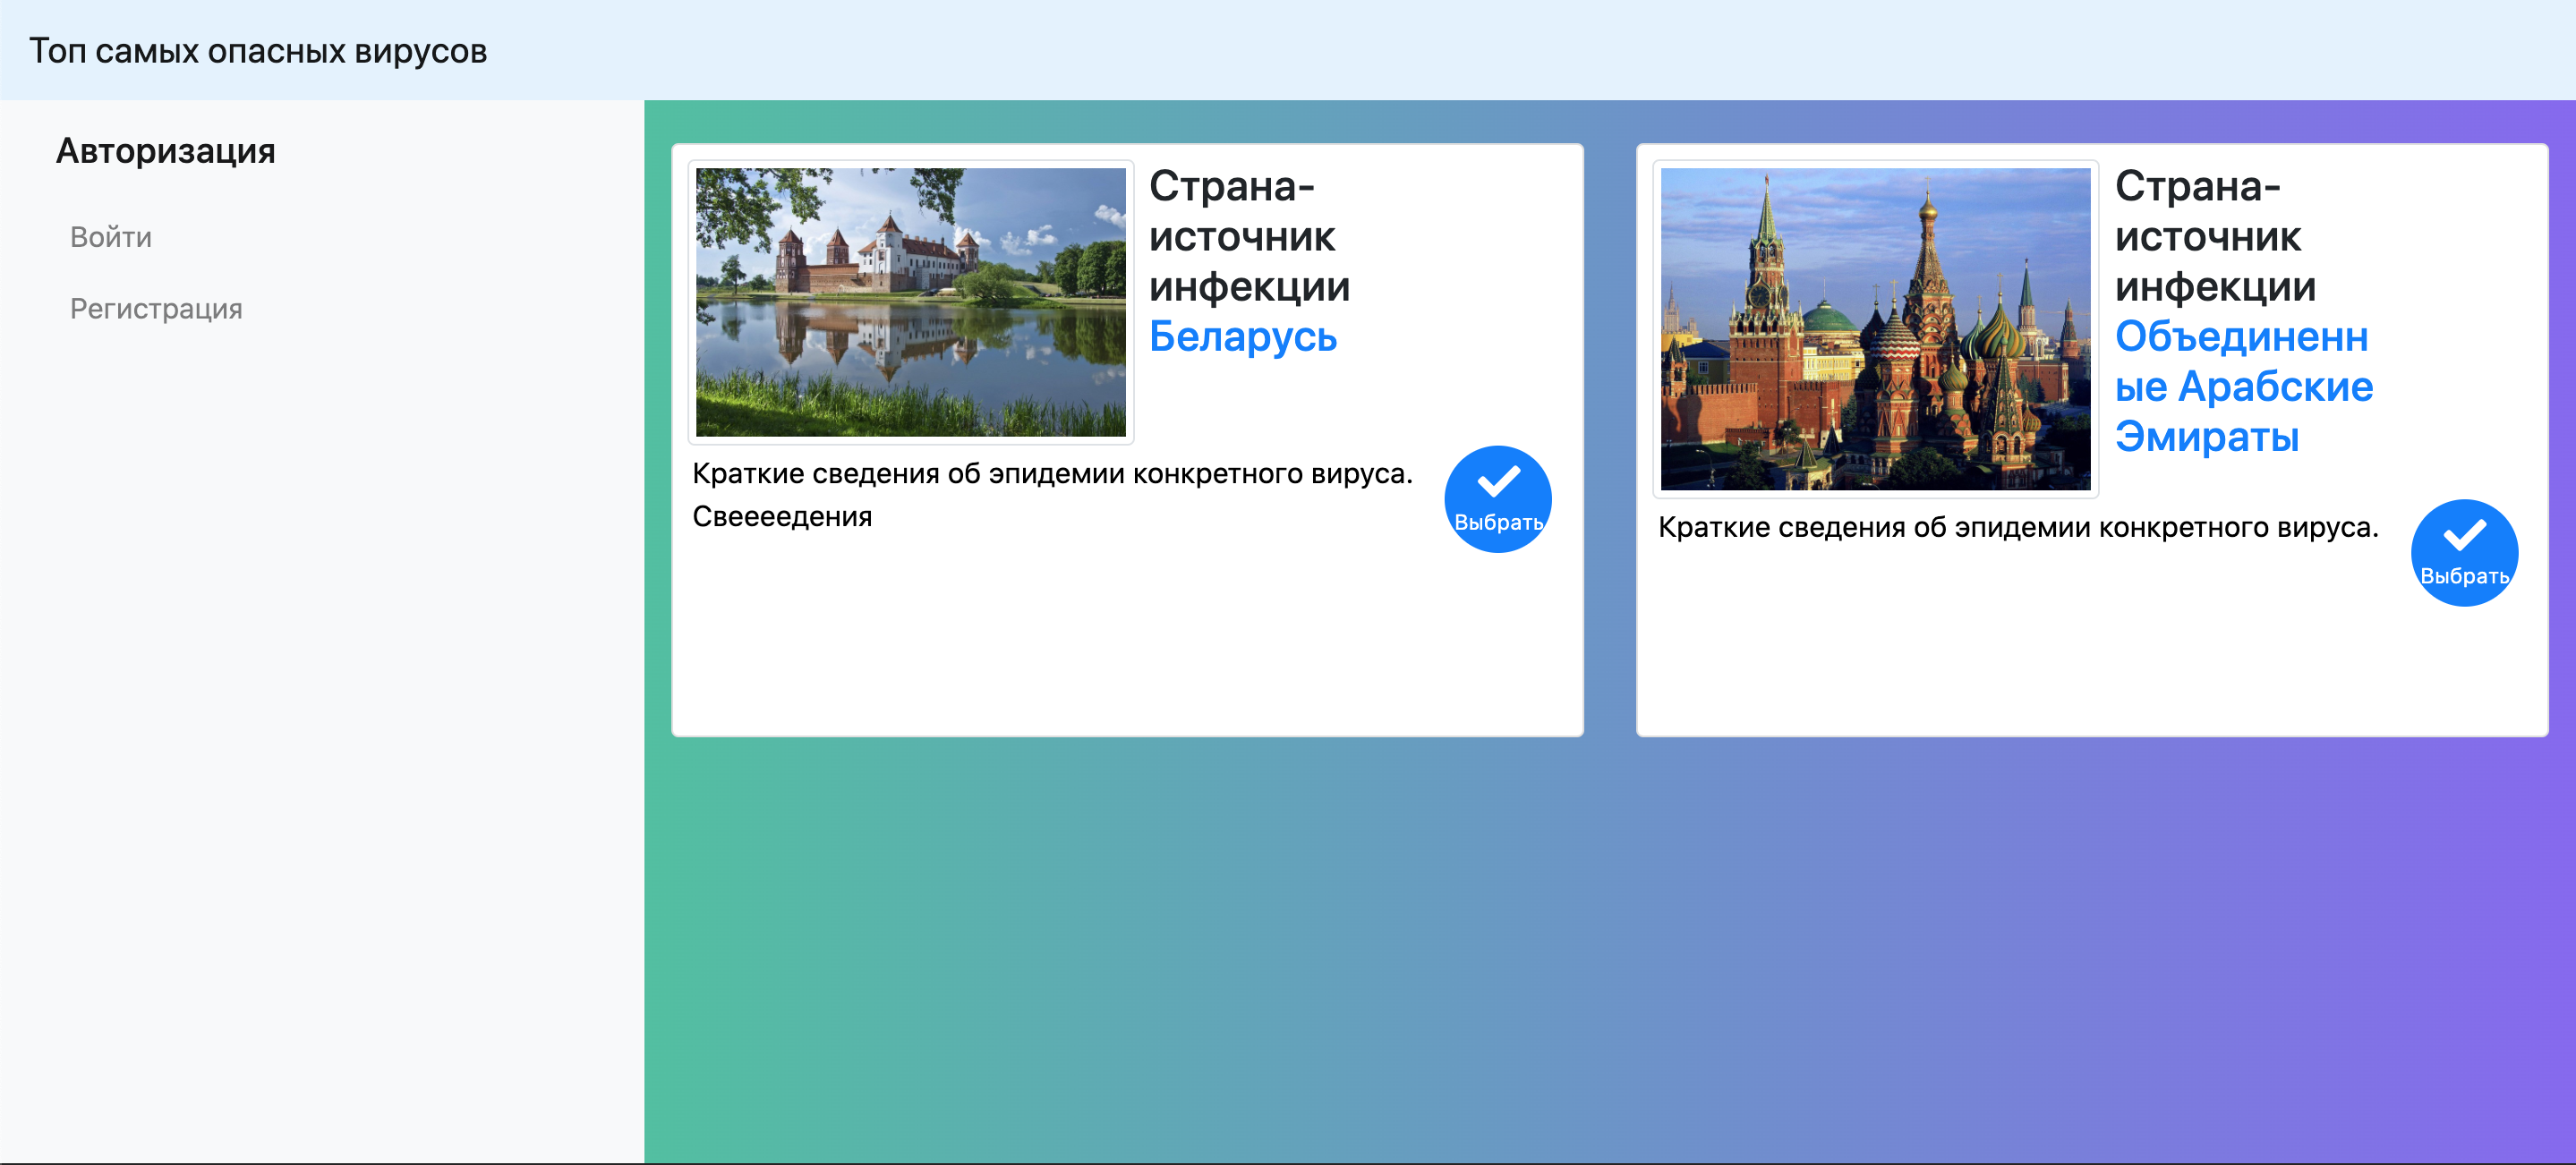
\includegraphics[width=\textwidth]{examples/epidemic.png}
 			\center{Список эпидемий}
 		\end{minipage}
 		\begin{minipage}[b]{0.45\textwidth}
 			
\includegraphics[width=\textwidth]{examples/region.png}
 			\center{Список регионов}
 		\end{minipage}
 		\label{ris:epidemic_region}
 	\end{figure}
 
 	\begin{figure}[h!]
 		\begin{minipage}[b]{0.45\textwidth}
 			
\includegraphics[width=\textwidth]{examples/country.png}
 			\center{Список стран}
 		\end{minipage}
 		\begin{minipage}[b]{0.45\textwidth}
 			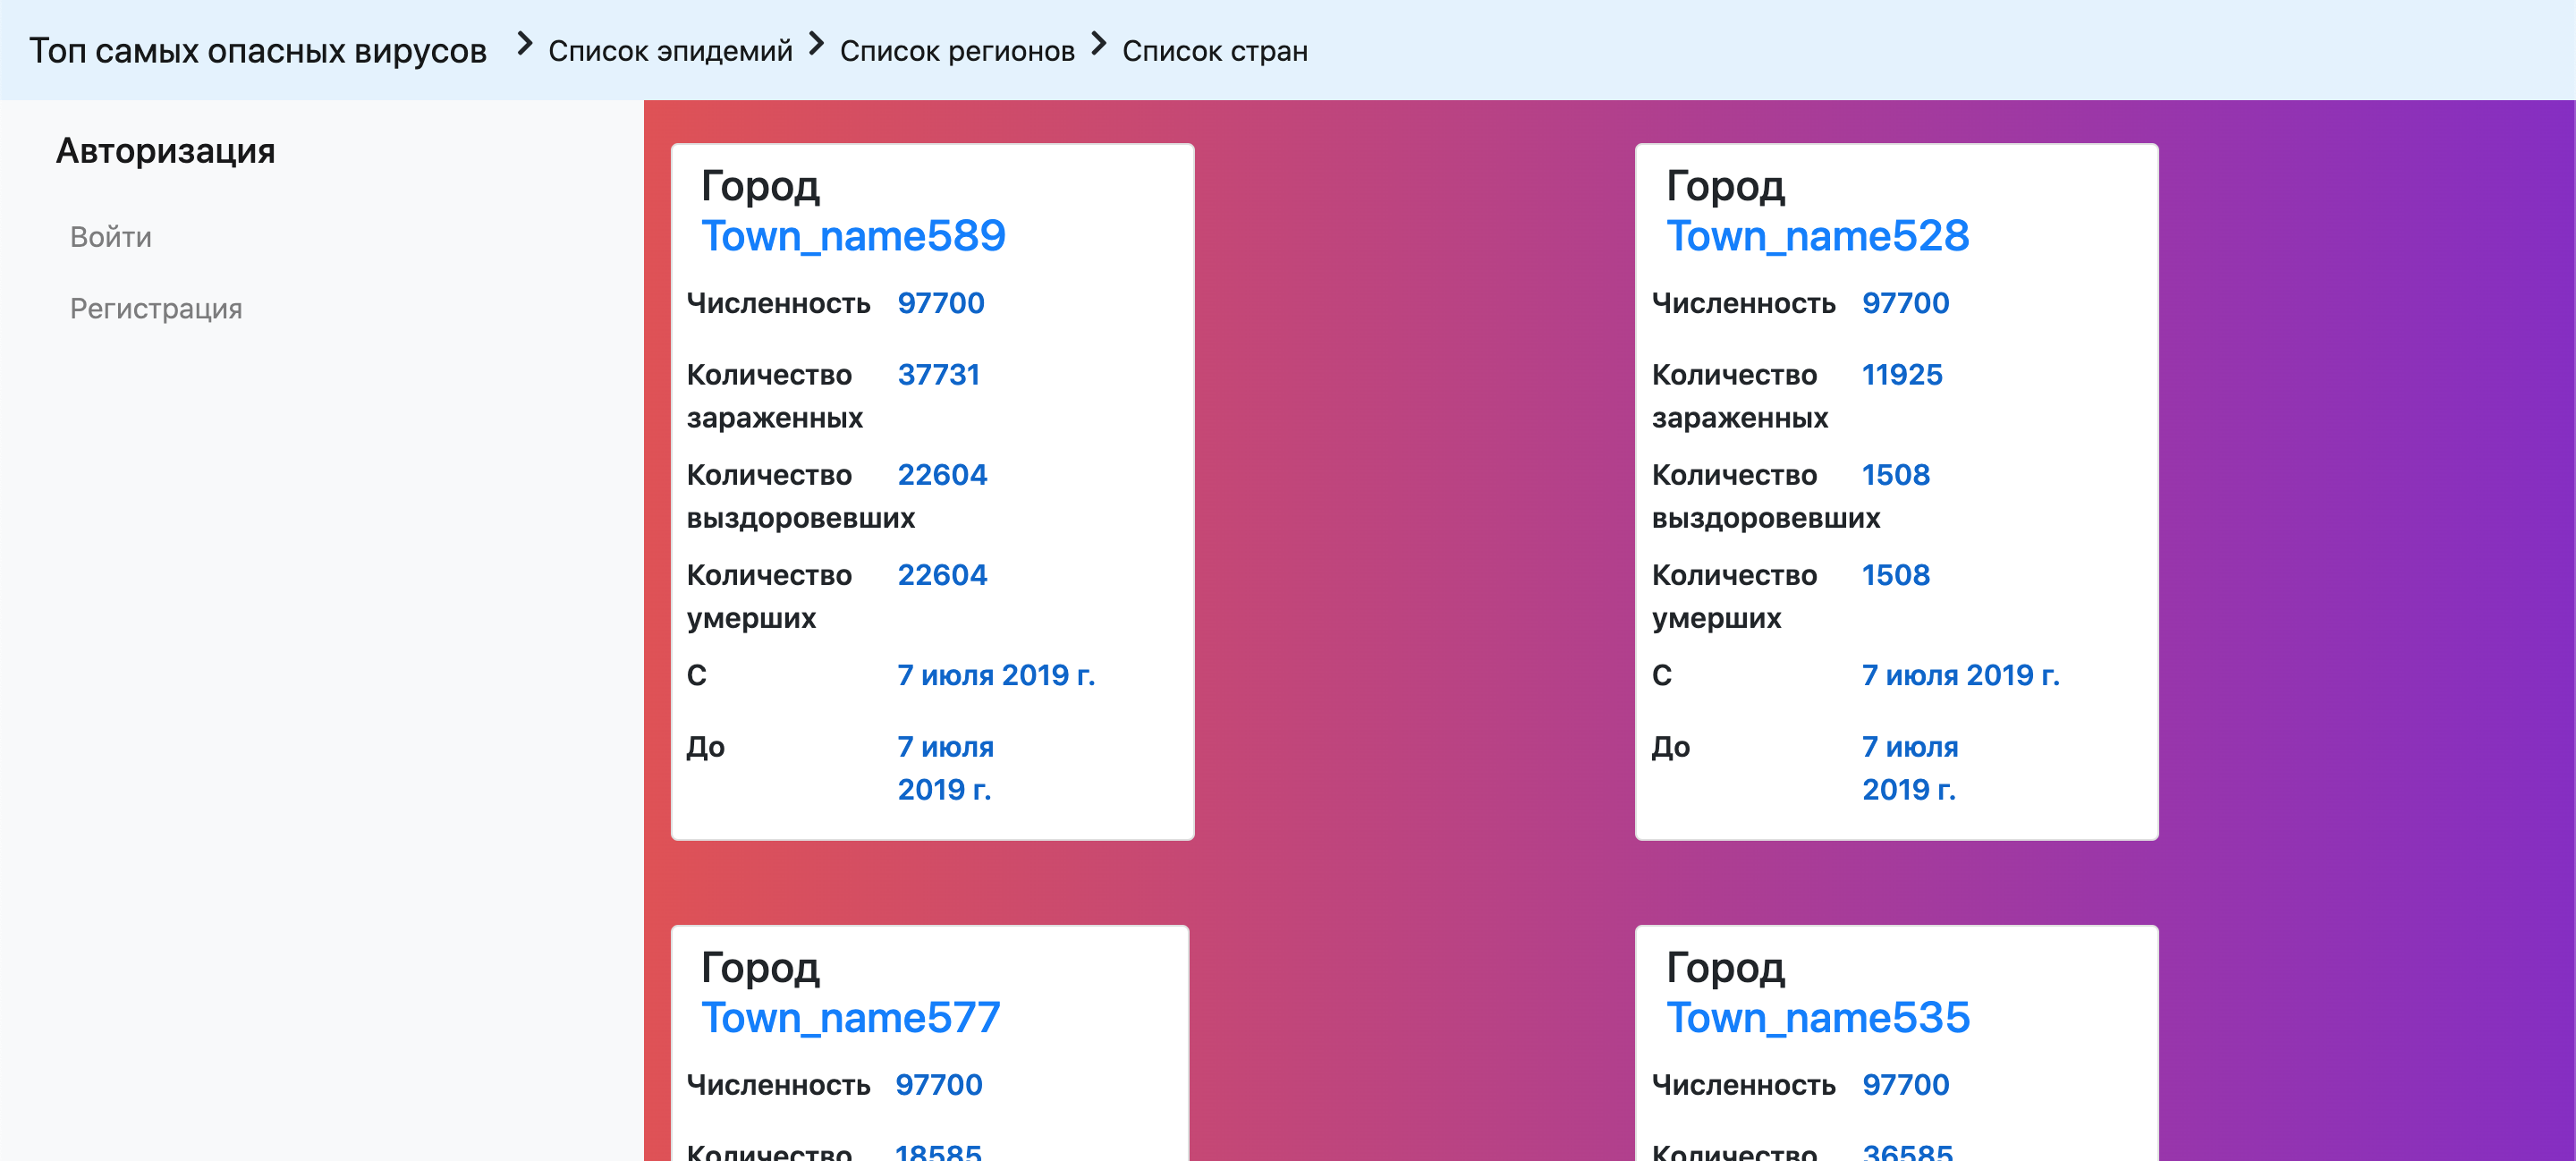
\includegraphics[width=\textwidth]{examples/town.png}
 			\center{Список городов}
 		\end{minipage}
 		\label{ris:country_town}
 	\end{figure}
 
 	Также, нажав на название какого-либо вируса или эпидемии, можно получить более подробную информацию о нем:
 	
 	\begin{figure}[h!]
 		\begin{center}
 			{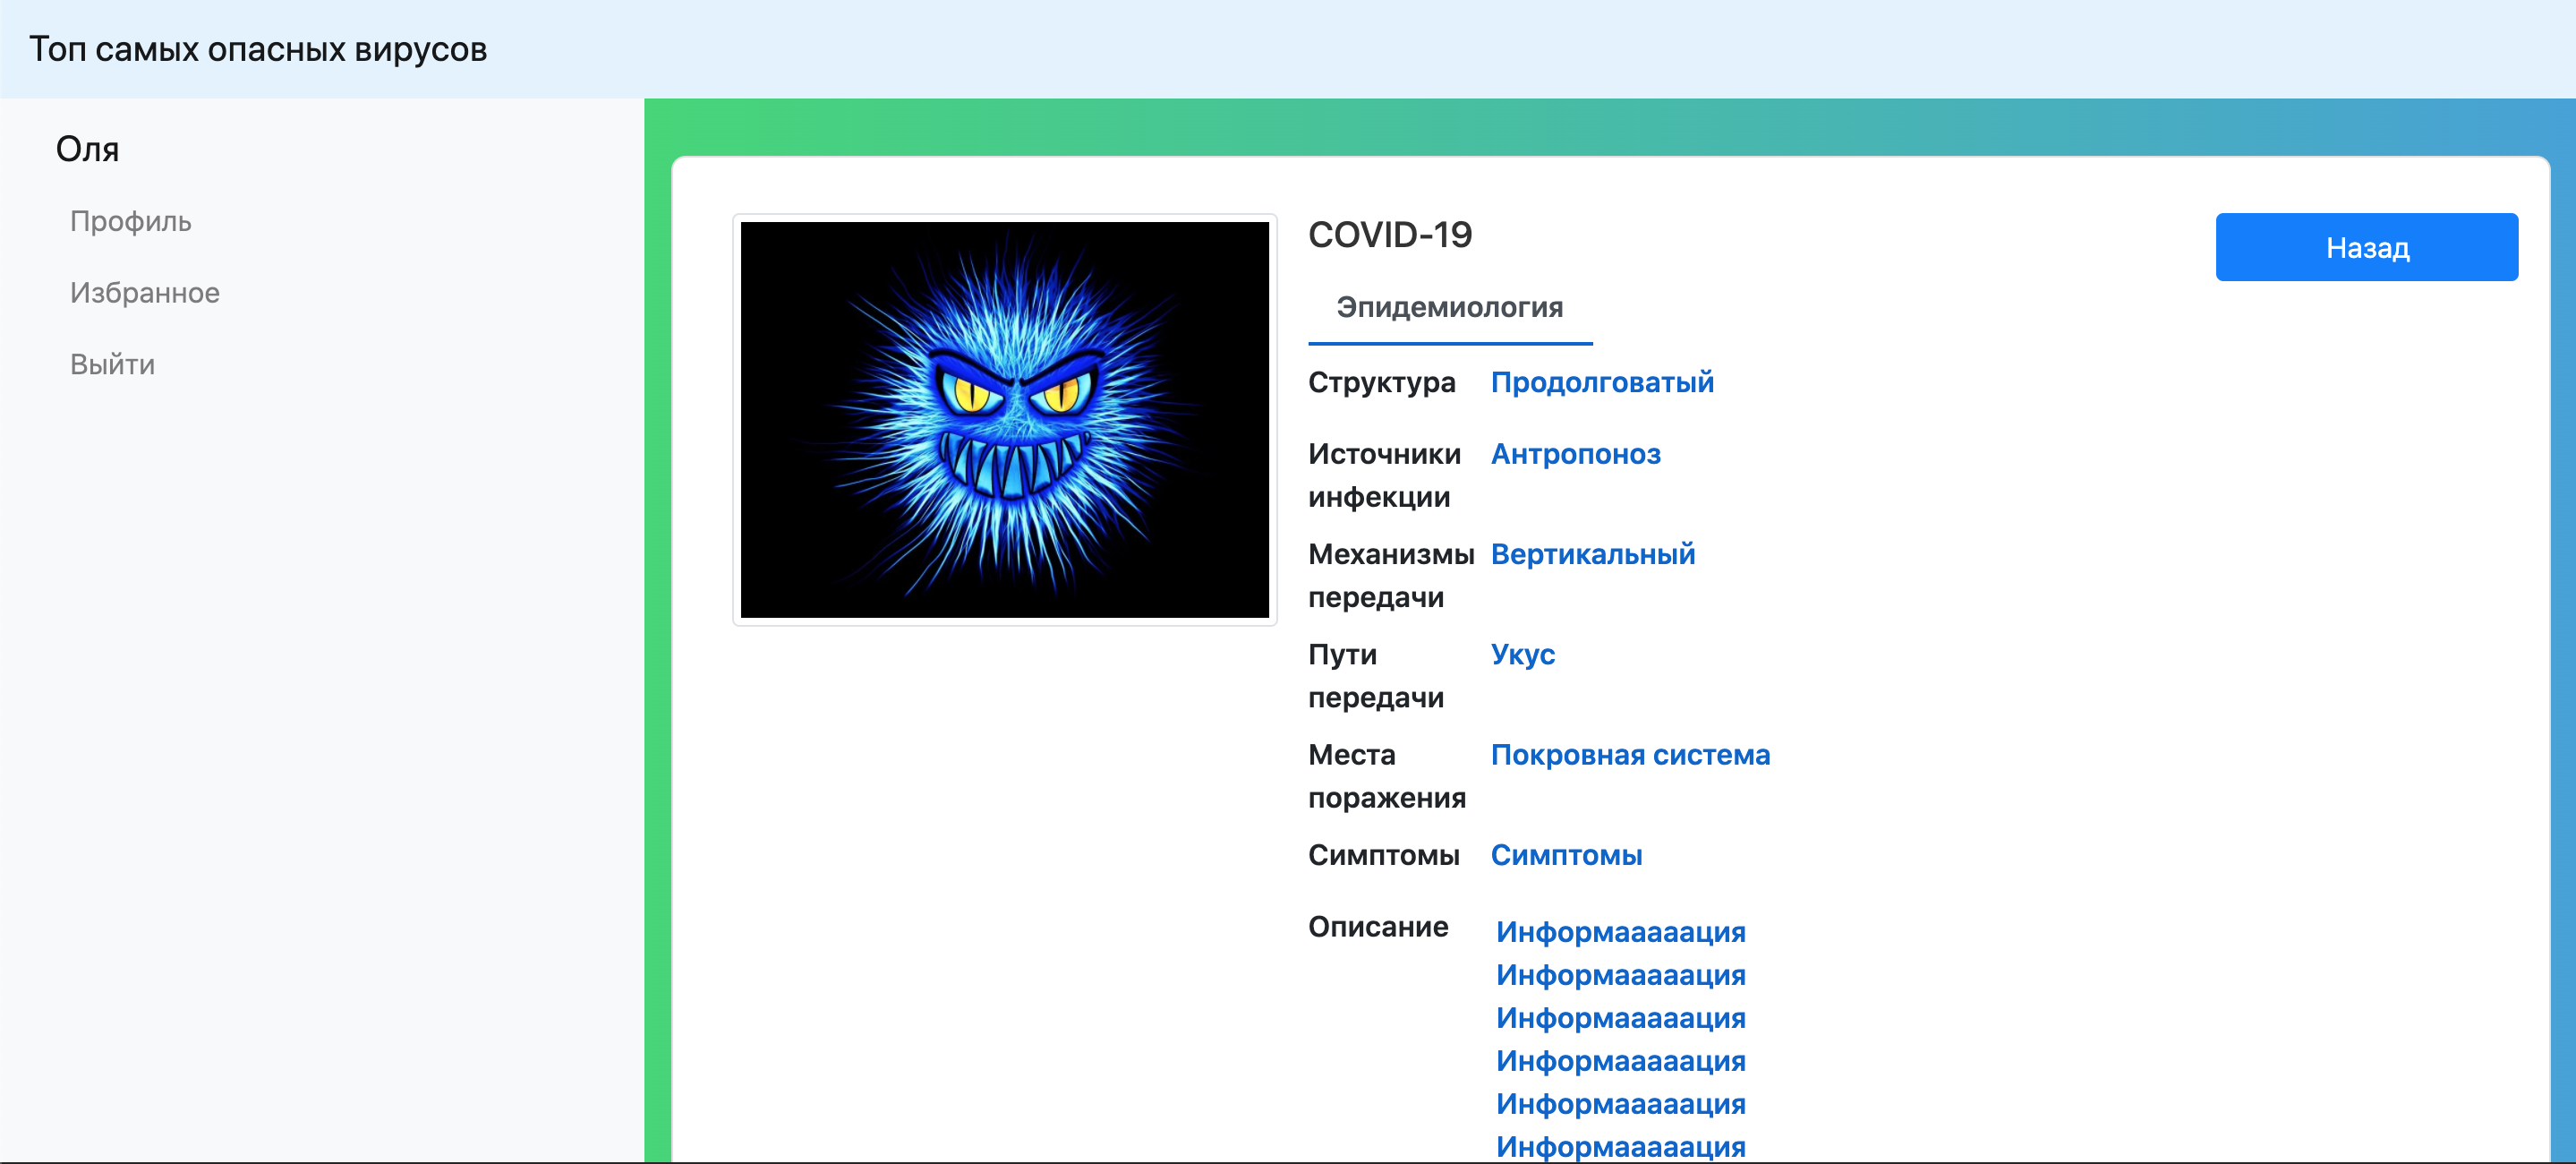
\includegraphics[width = \textwidth]{examples/more_virus.png}}
 			\caption{
 				Подробная информация о вирусе}
 			\label{ris:more_virus}
 		\end{center}
 	\end{figure}
 
 	\newpage
 
 	На любой из перечисленных страниц можно увидеть слева панель, на которой будет предложено либо войти пользователю либо зарегистрироваться:
 
	 \begin{figure}[h!]
	 	\begin{minipage}[b]{0.45\textwidth}
	 		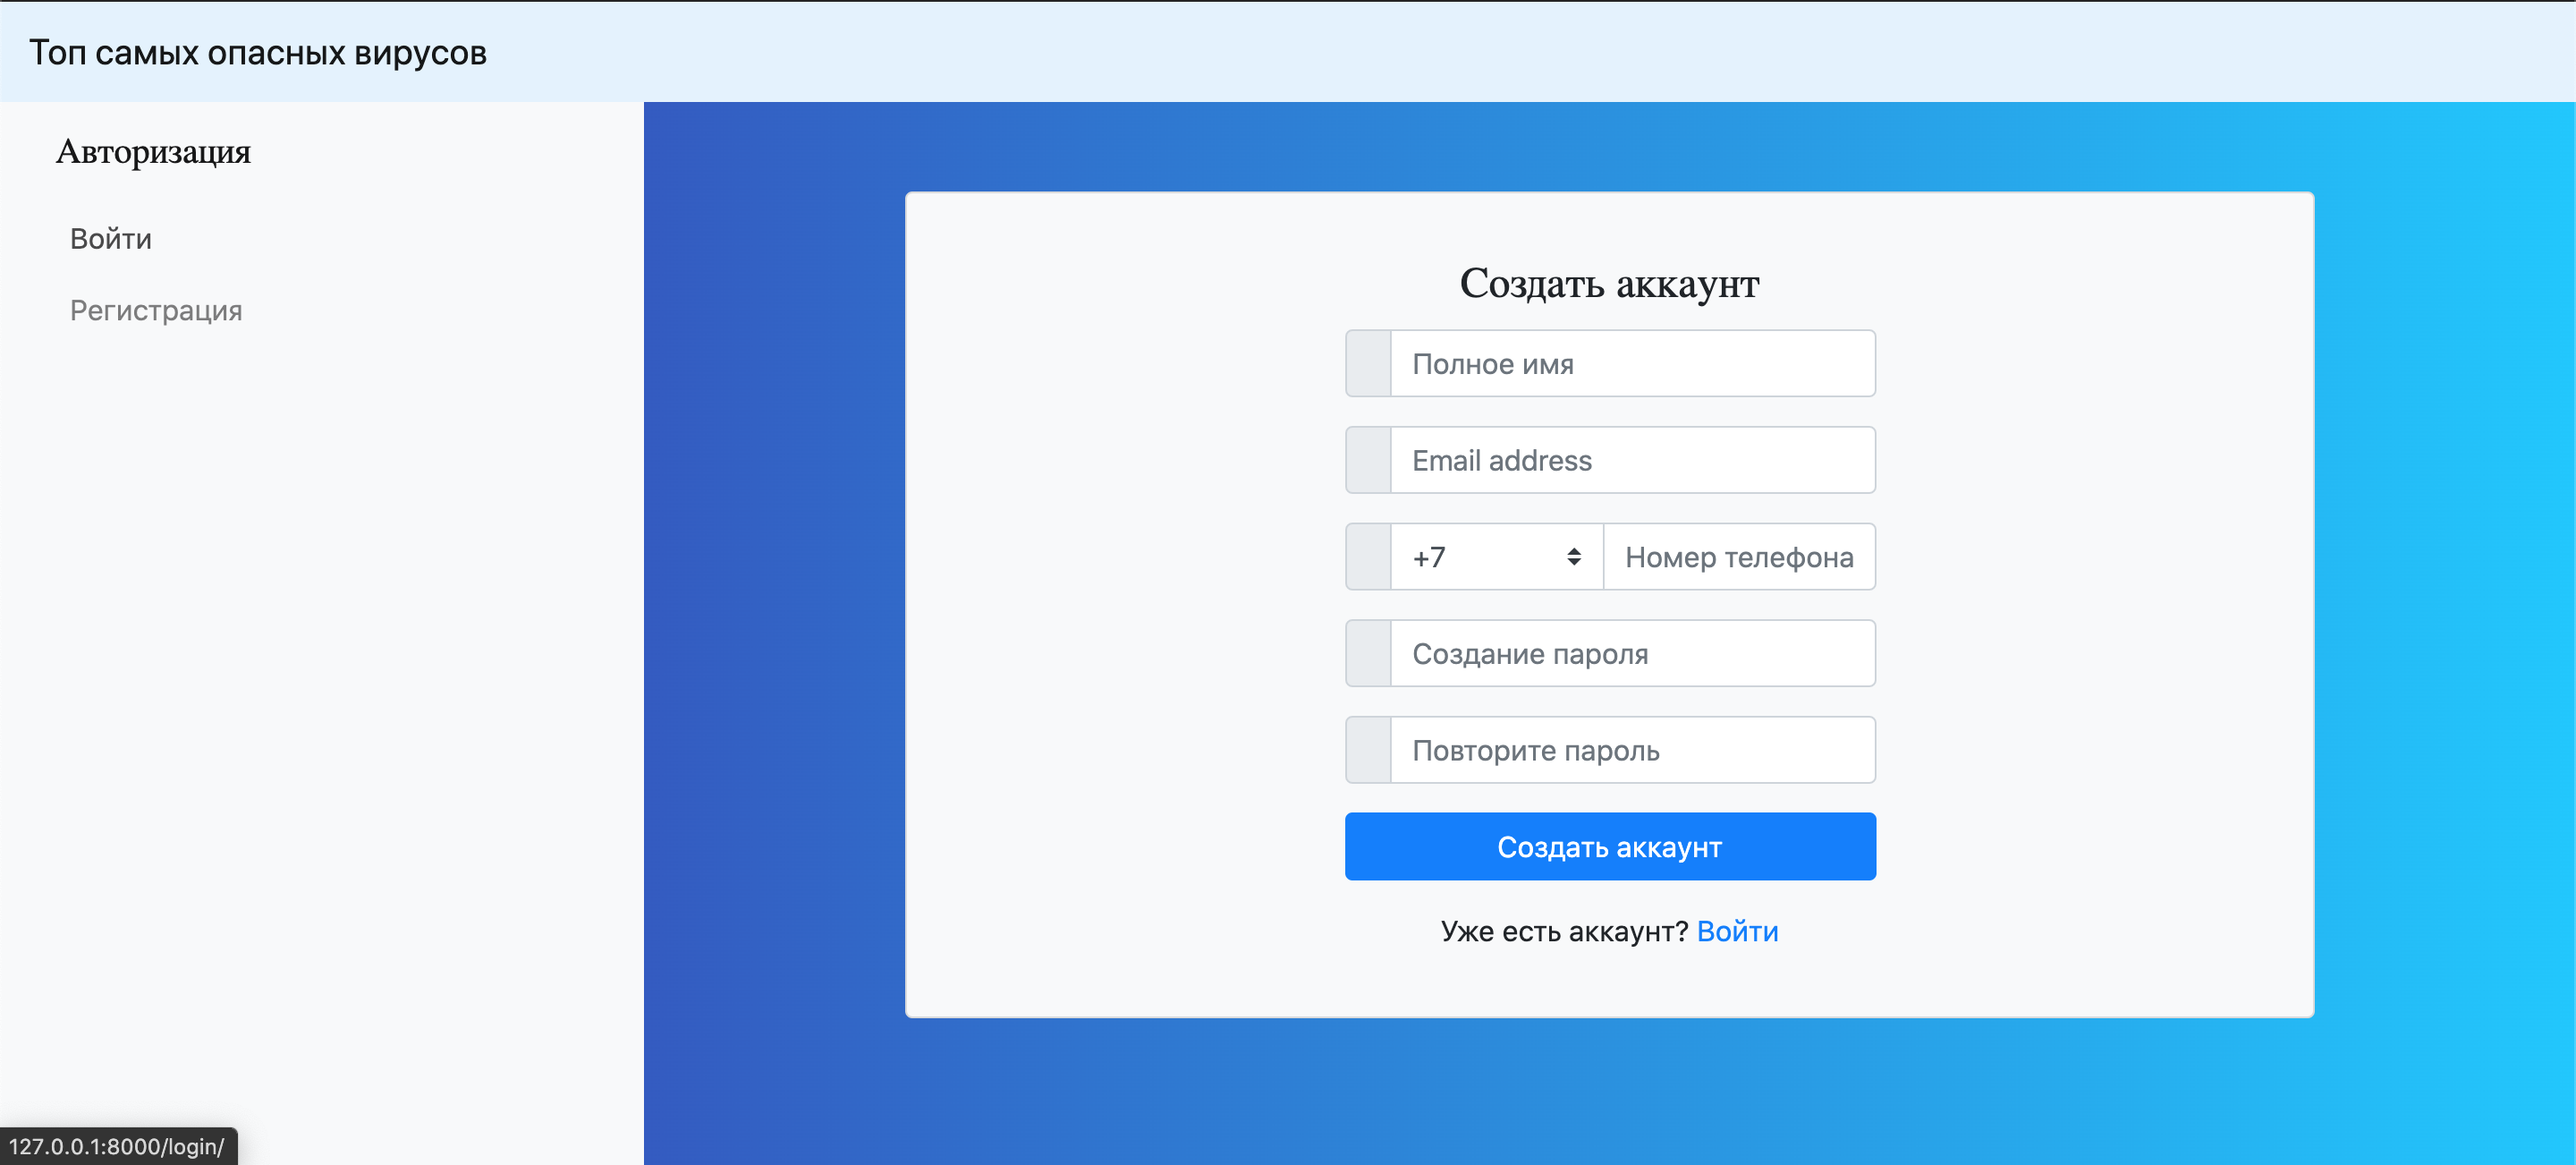
\includegraphics[width=\textwidth]{examples/register.png}
	 		\center{Страница регистрации}
	 	\end{minipage}
	 	\begin{minipage}[b]{0.45\textwidth}
	 		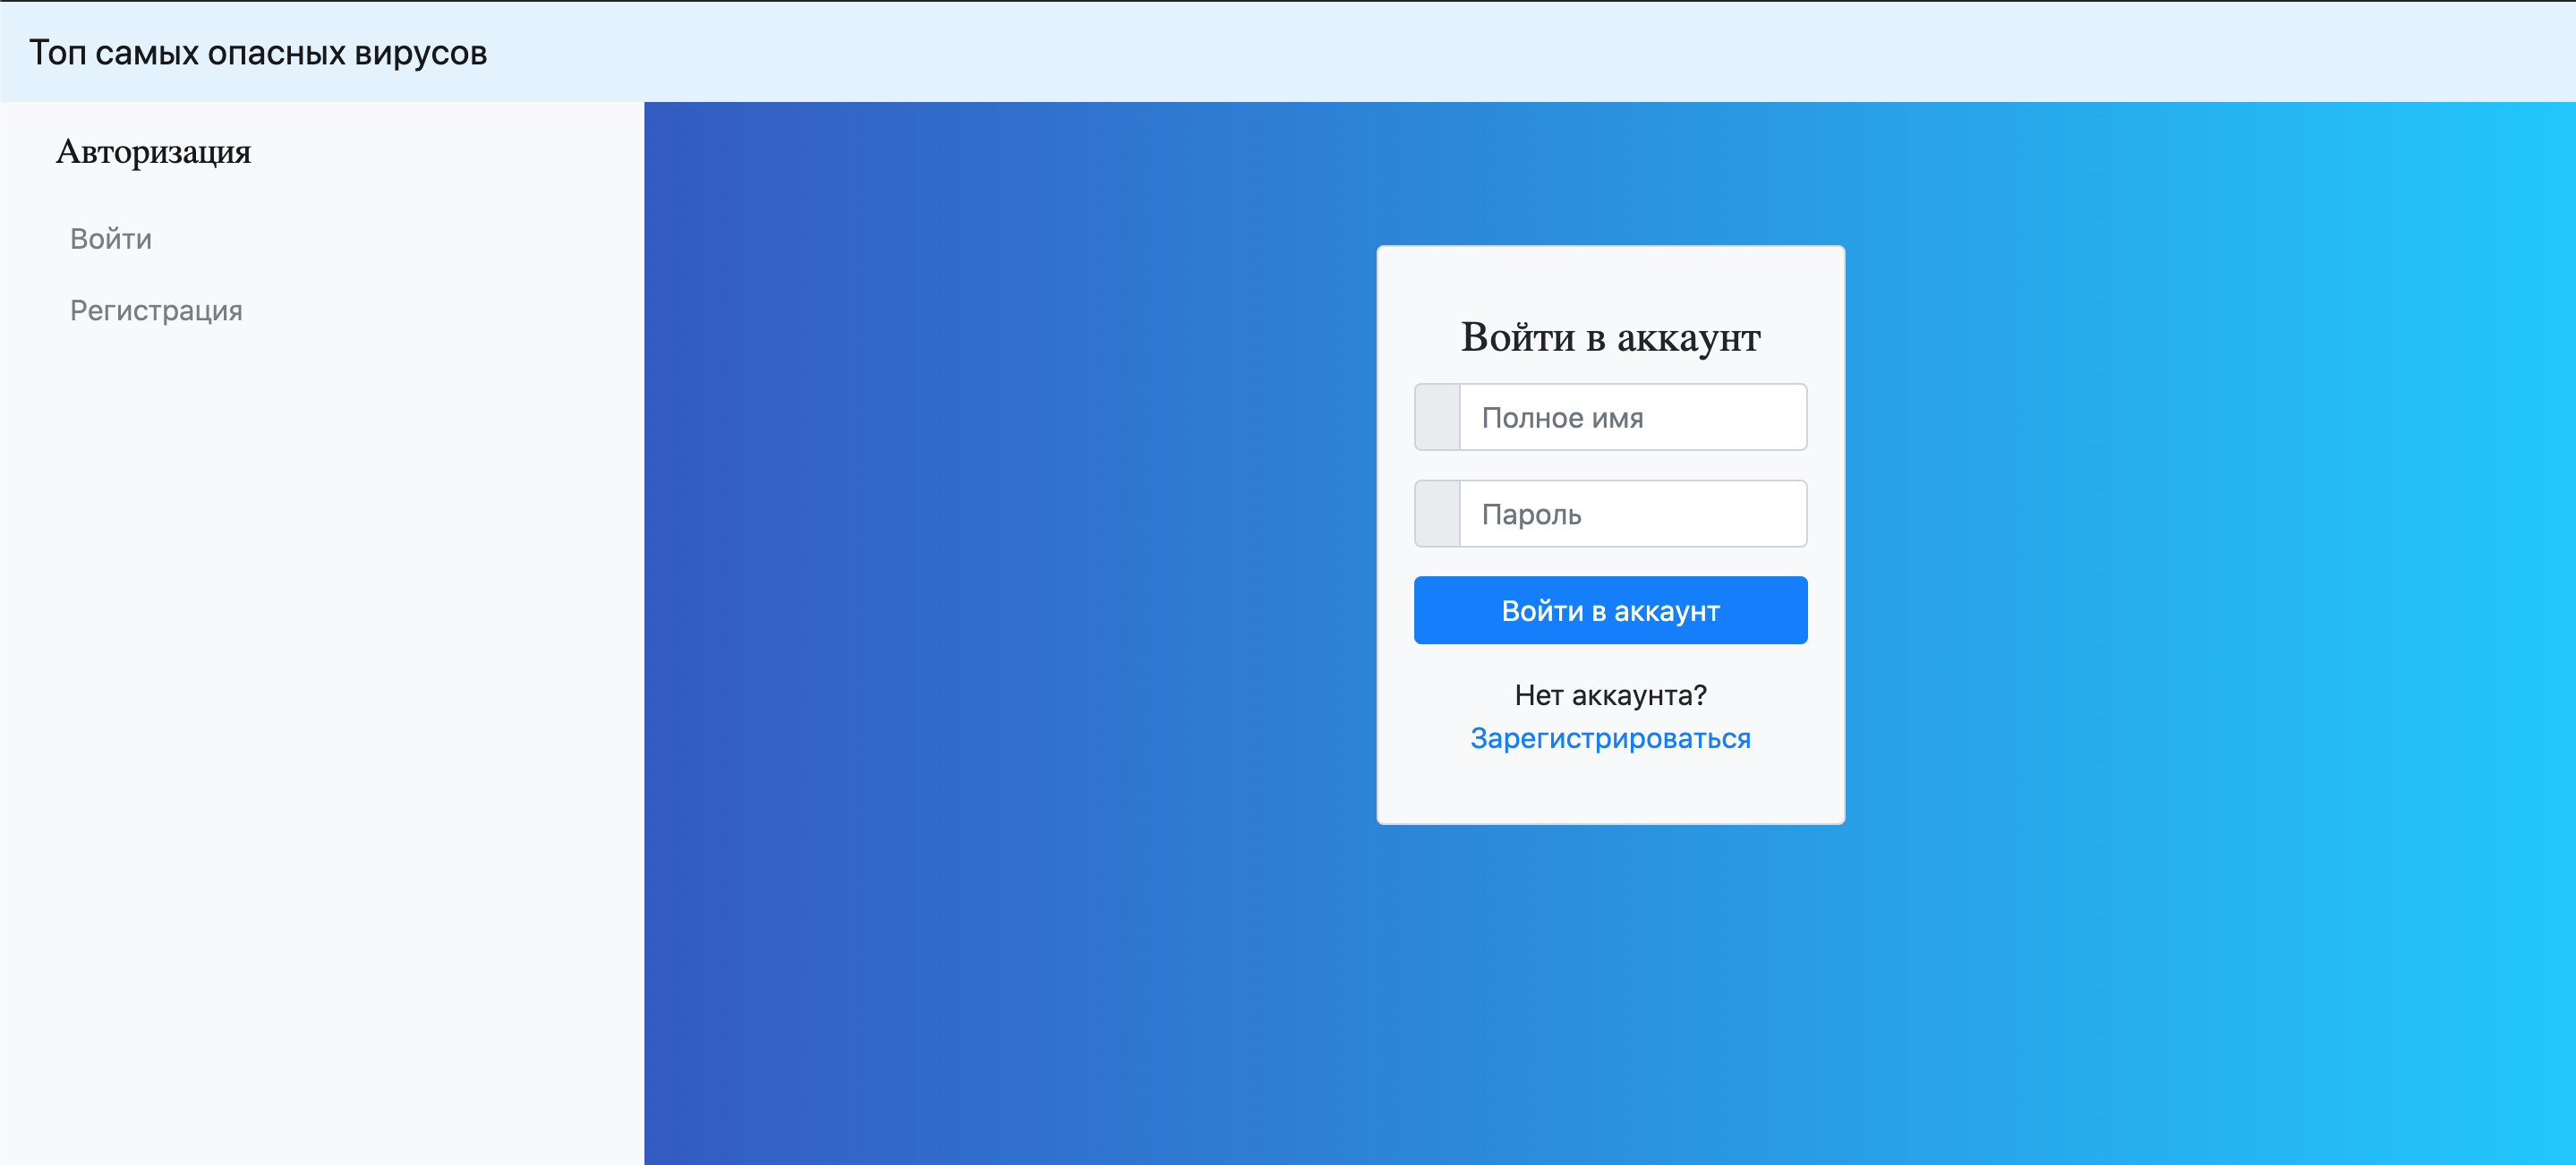
\includegraphics[width=\textwidth]{examples/login.png}
	 		\center{Страница входа в систему}
	 	\end{minipage}
	 	\label{ris:register_login}
	 \end{figure}
 
 	Далее, после прохождения регистрации/входа в систему пользователя перекидывает на страницу его профиля, который можно отредактировать, добавив более подробную информацию о себе.
 	
 	\begin{figure}[h!]
 		\begin{minipage}[b]{0.45\textwidth}
 			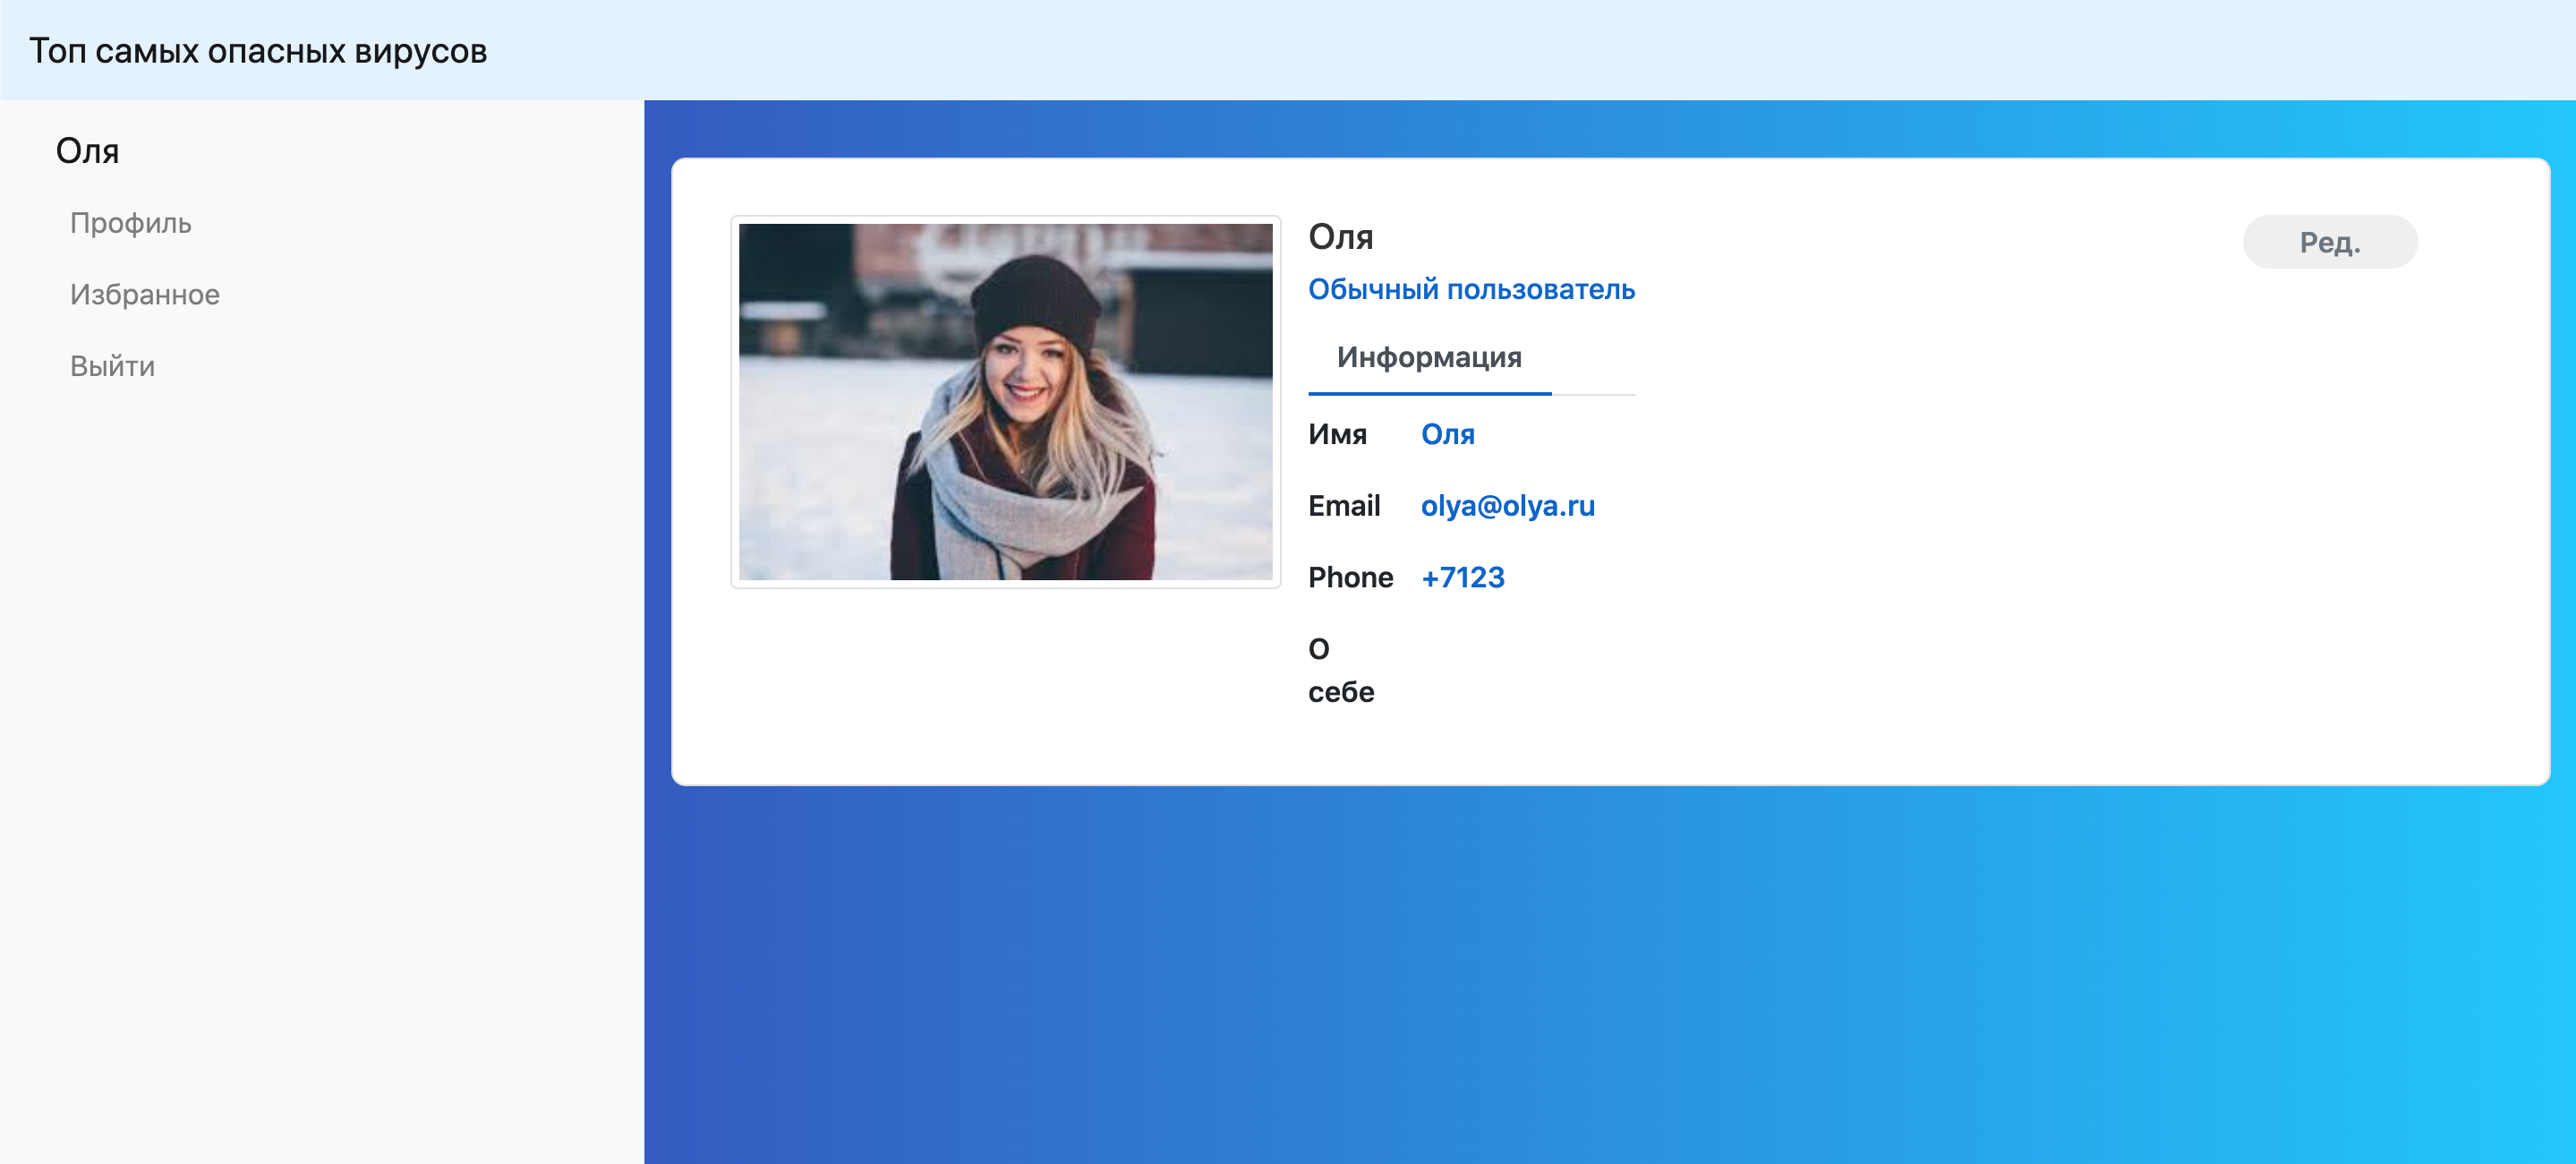
\includegraphics[width=\textwidth]{examples/profile.png}
 			\center{Профиль}
 		\end{minipage}
 		\begin{minipage}[b]{0.45\textwidth}
 			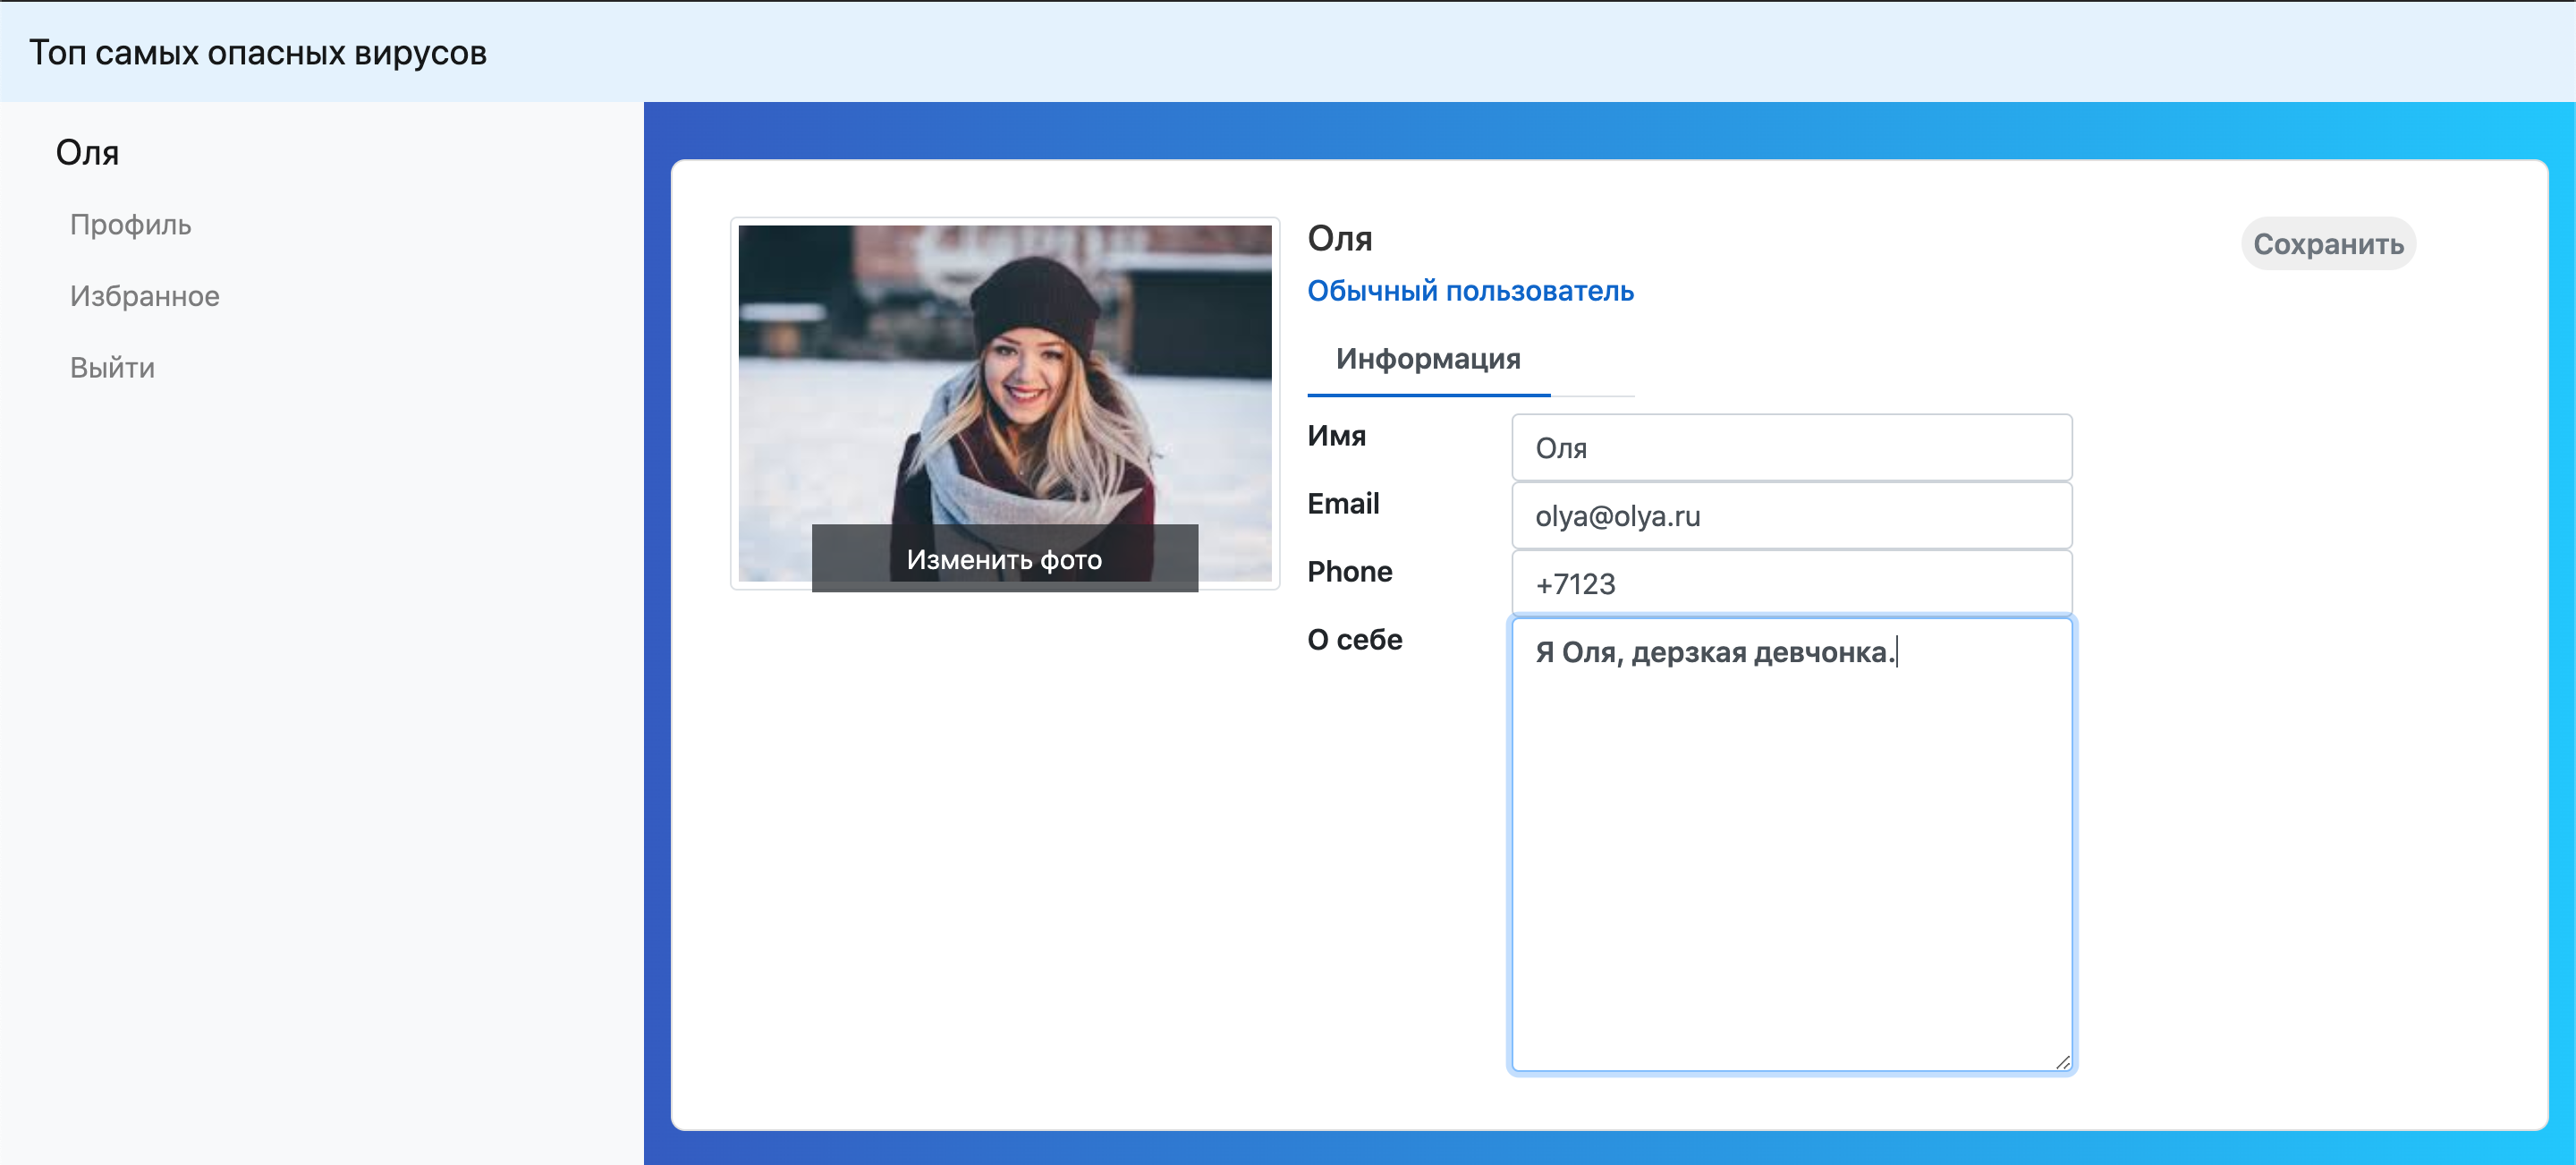
\includegraphics[width=\textwidth]{examples/edit_profile.png}
 			\center{Редактирование профиля}
 		\end{minipage}
 		\label{ris:profile_edit_profile}
 	\end{figure}
 
 
 	При переходе на главную страницу сайта можно заметить, что на карточках с информацией о вирусах появились новые иконки - звездочки. Именно с помощью них осуществляется добавление и удаление из избранного понравившейся информации конкретному пользователю.
 
 	\begin{figure}[h!]
 		\begin{minipage}[b]{0.45\textwidth}
 			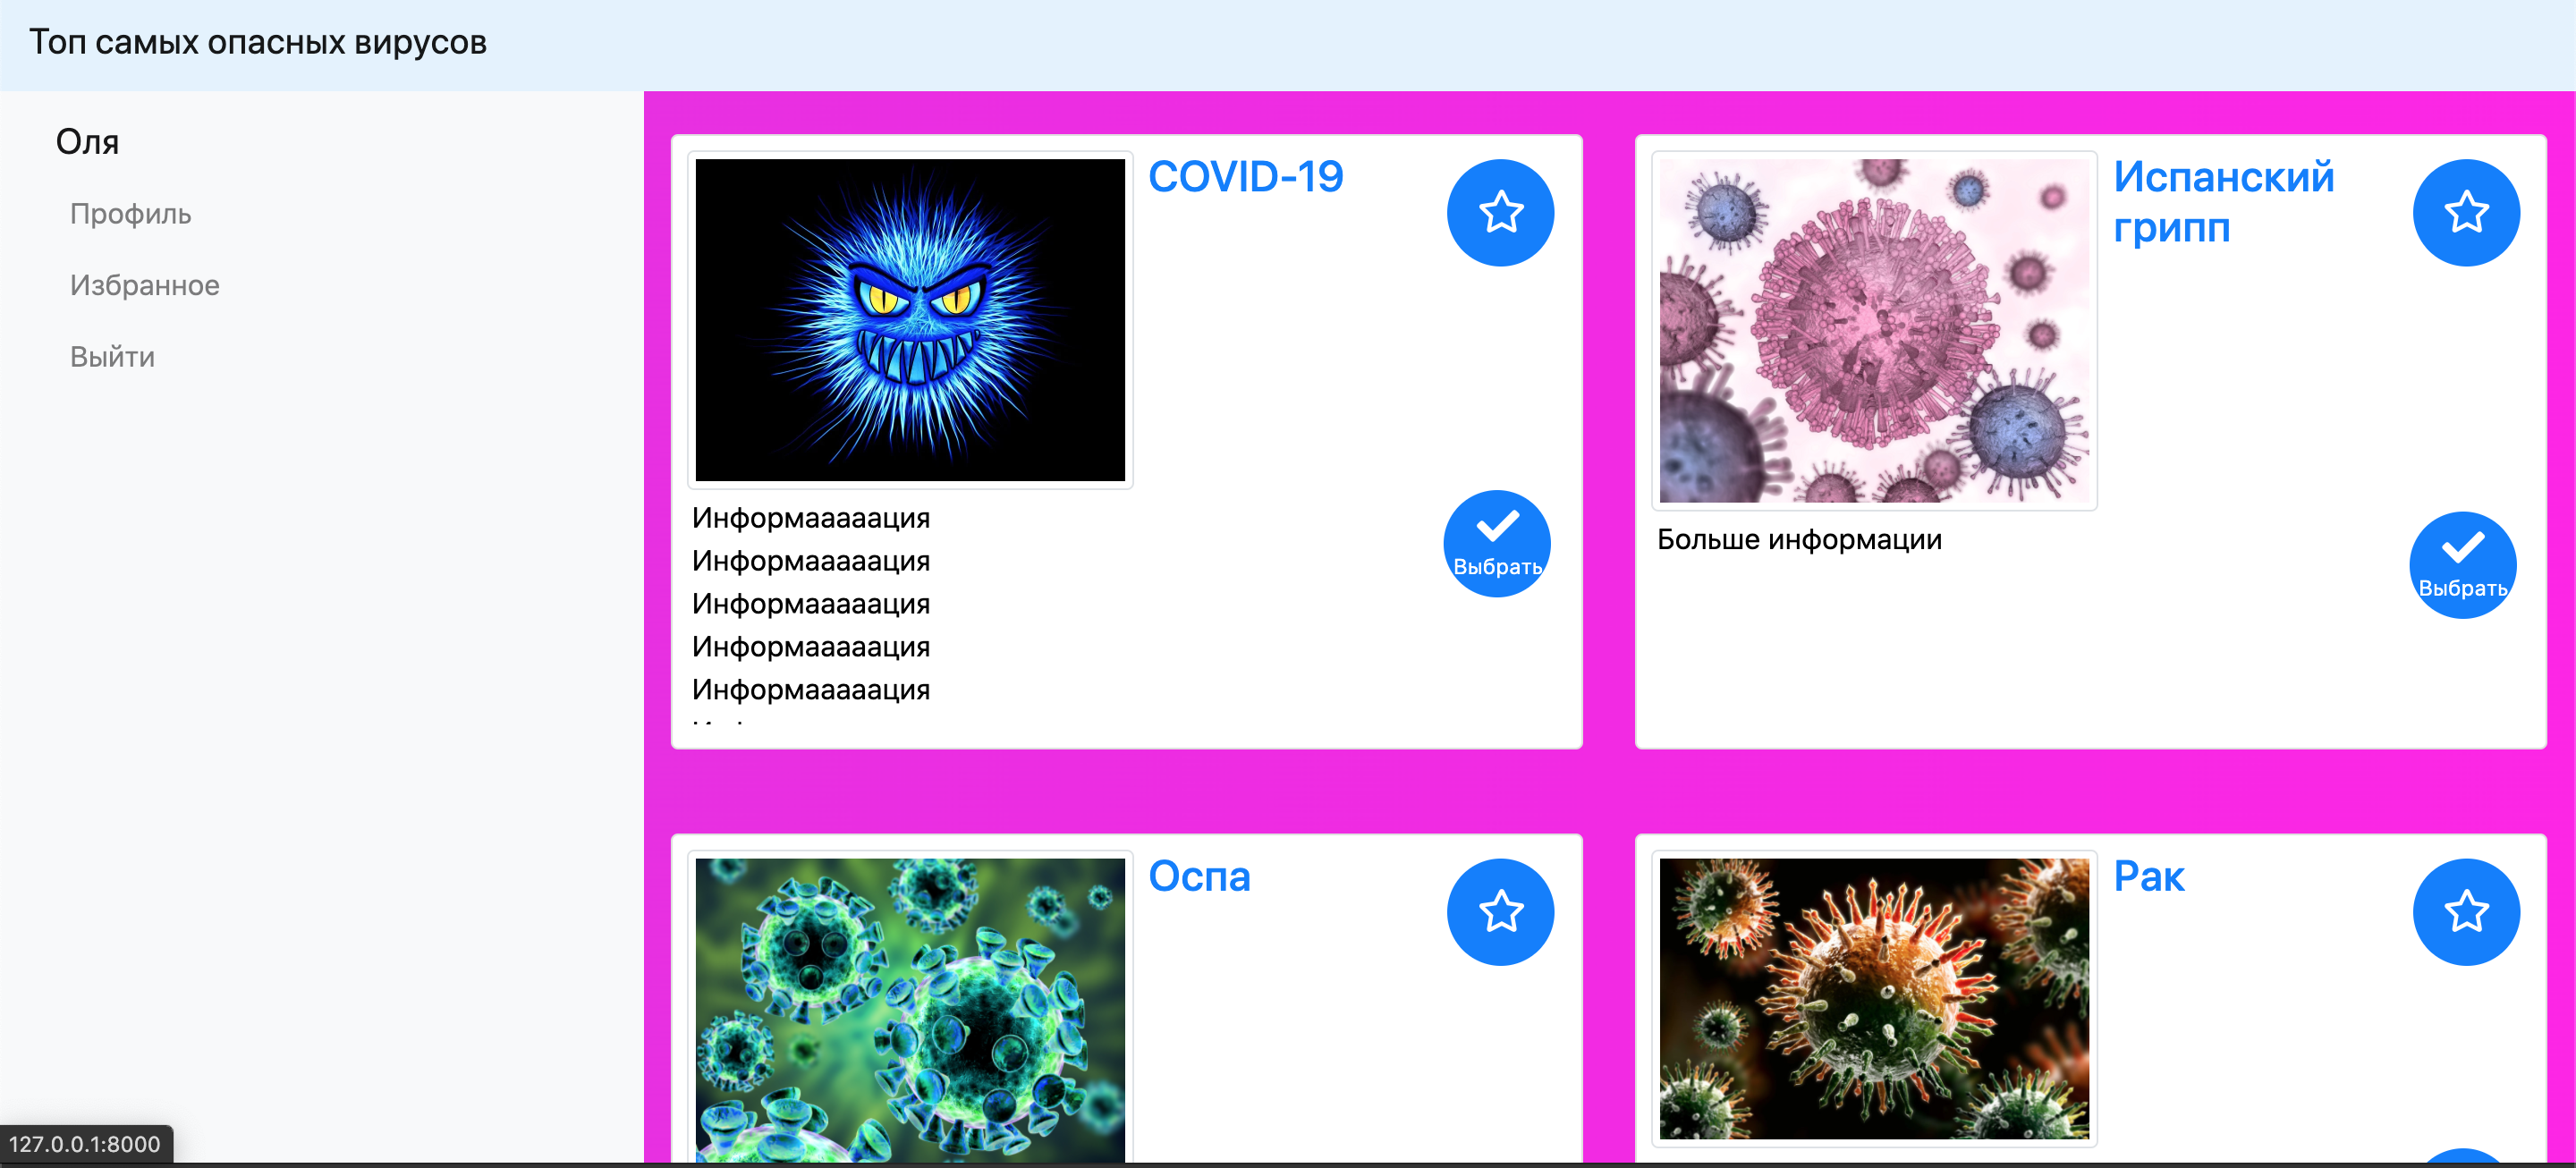
\includegraphics[width=\textwidth]{examples/stars.png}
 			\center{Главная страница (список вирусов) с возможностью добавлять элементы в избранное}
 		\end{minipage}
 		\begin{minipage}[b]{0.55\textwidth}
 			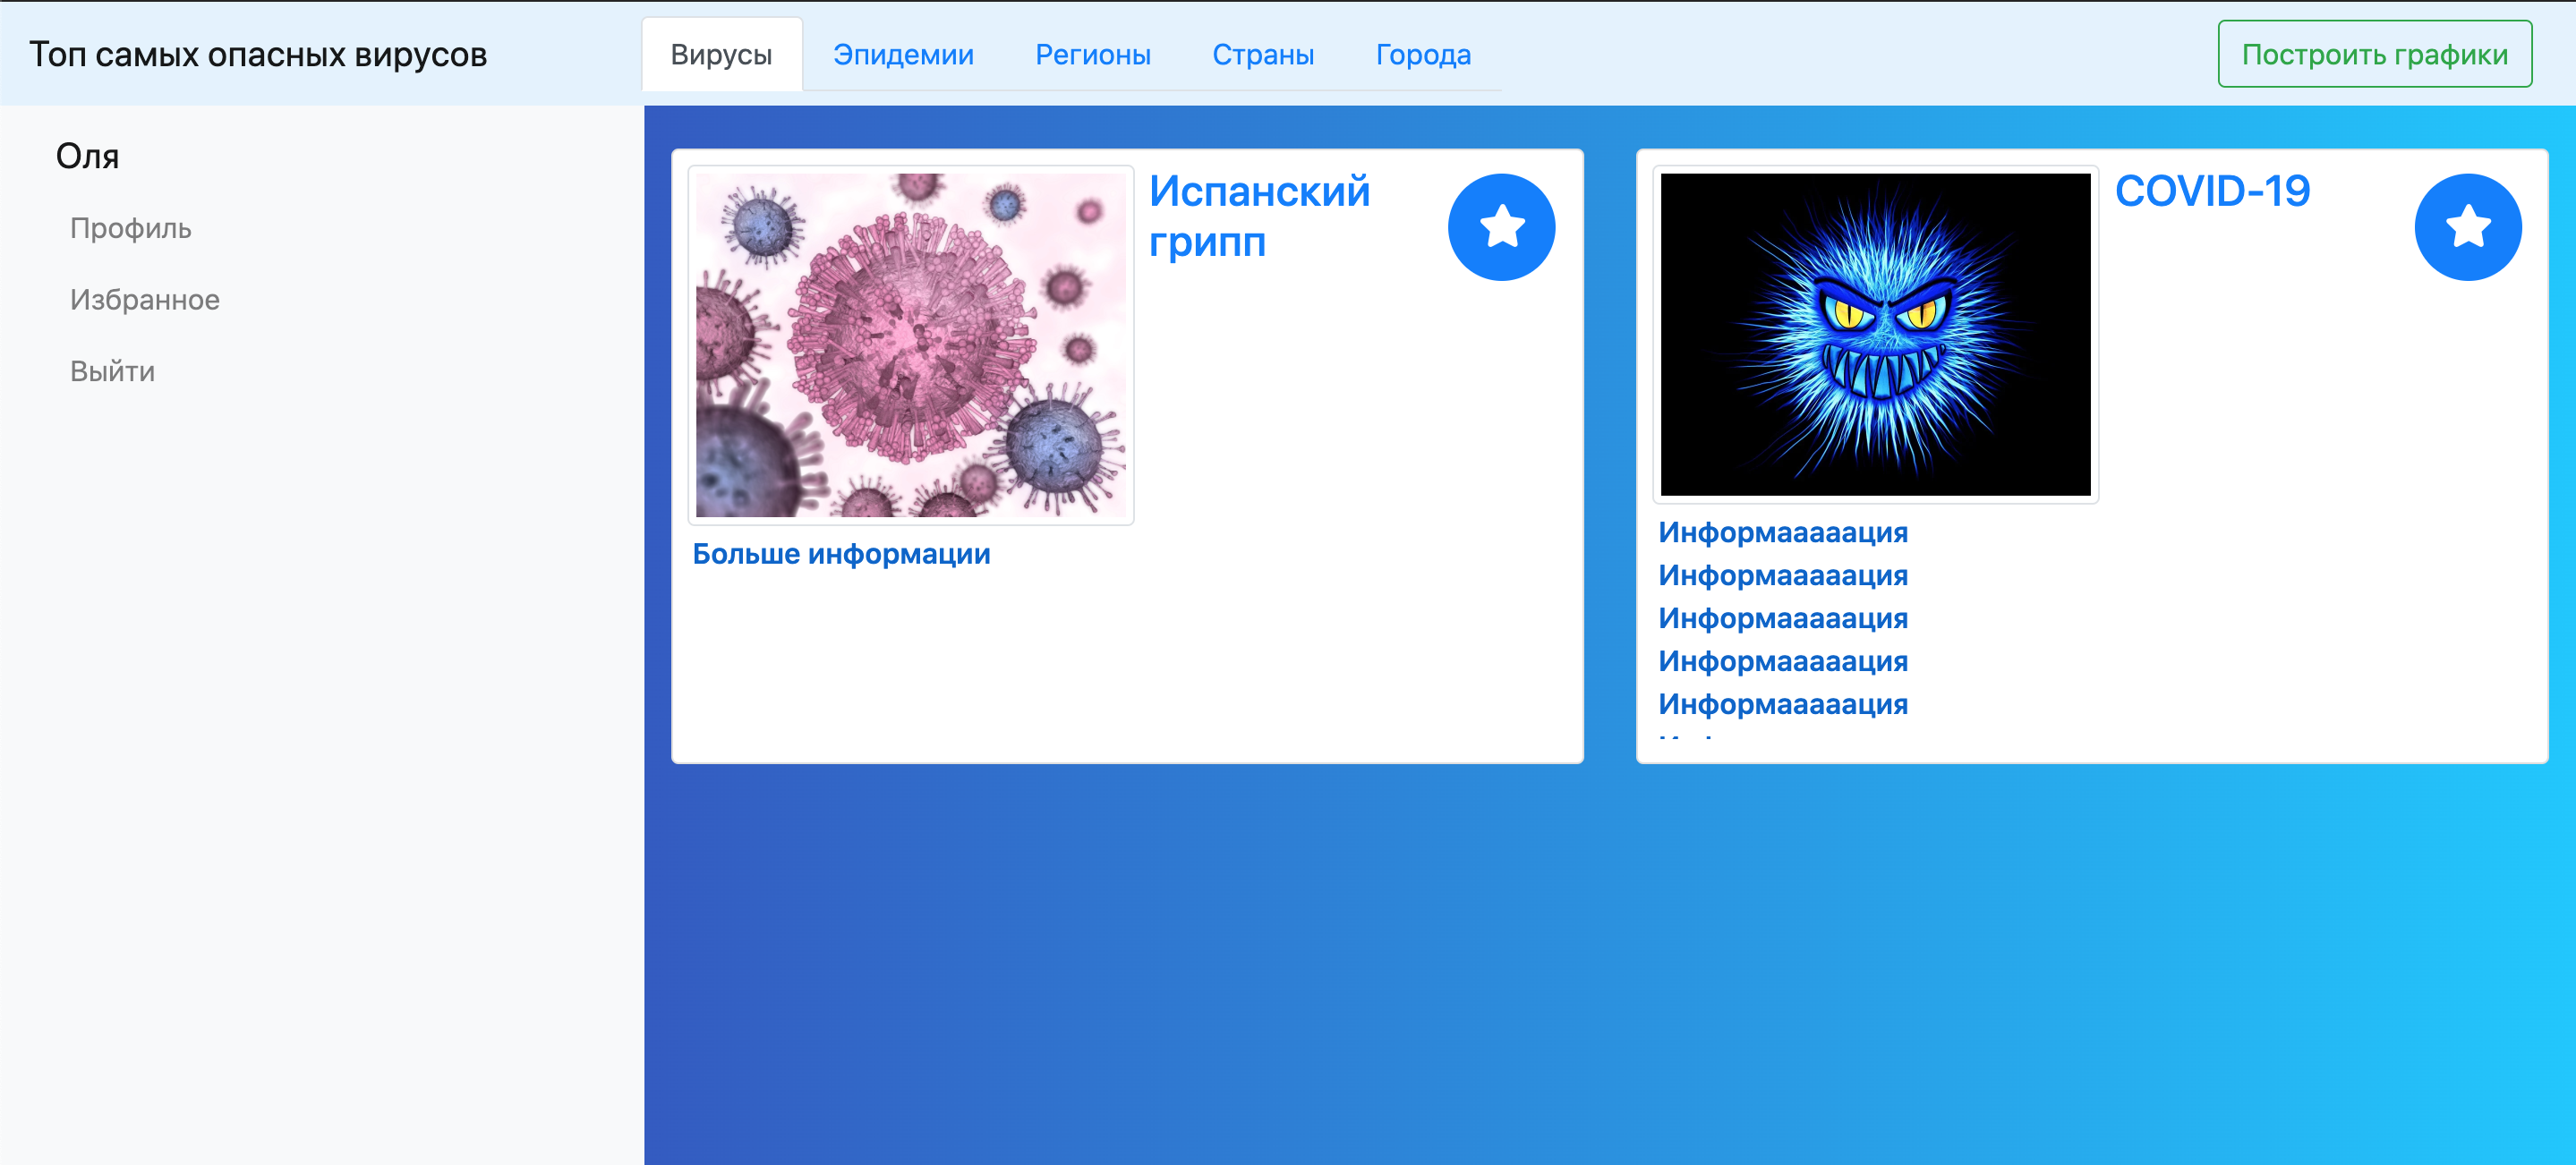
\includegraphics[width=\textwidth]{examples/favourties.png}
 			\center{Вирусы, попавшие в избранное}
 		\end{minipage}
 		\label{ris:stars_favourites}
 	\end{figure}
 
 	\newpage
 	
 	Перейдя во вкладку <<избранное>>, пользователь также сможет выбрать из добавленных им регионов, стран, городов те, что захочет проанализировать, и построить графики.
 	
 	\begin{figure}[h!]
 		\begin{center}
 			{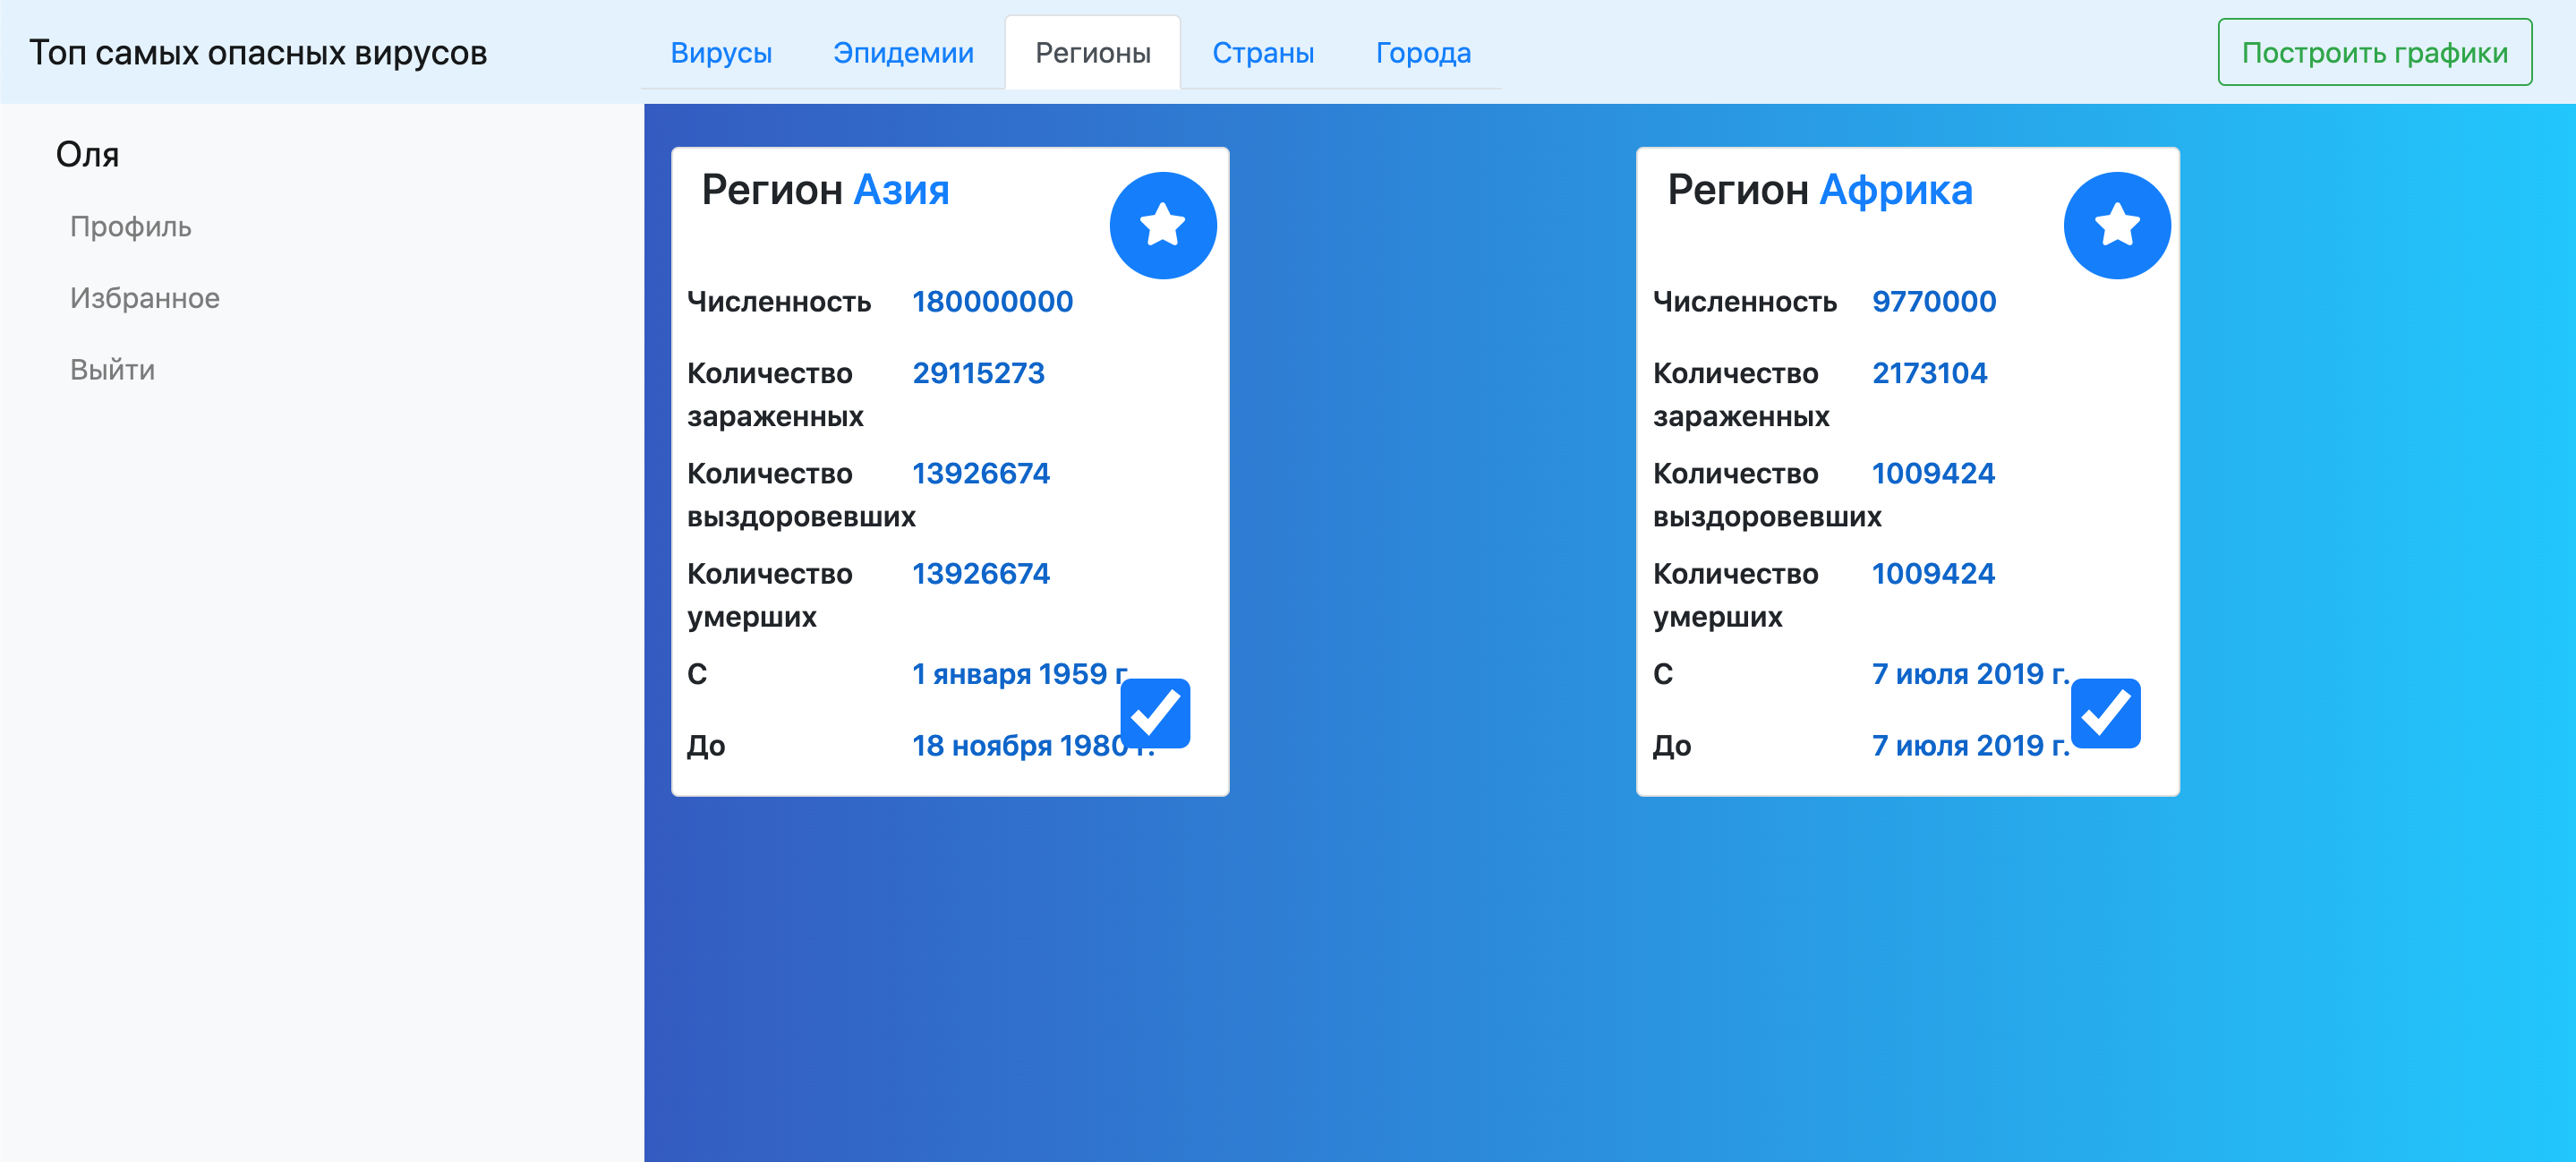
\includegraphics[width = \textwidth]{examples/favourite_regions.png}}
 			\caption{Регионы добавленные в избранное}
 			\label{ris:favourite_regions}
 		\end{center}
 	\end{figure}
 	
 	\begin{figure}[h!]
 		\begin{center}
 			{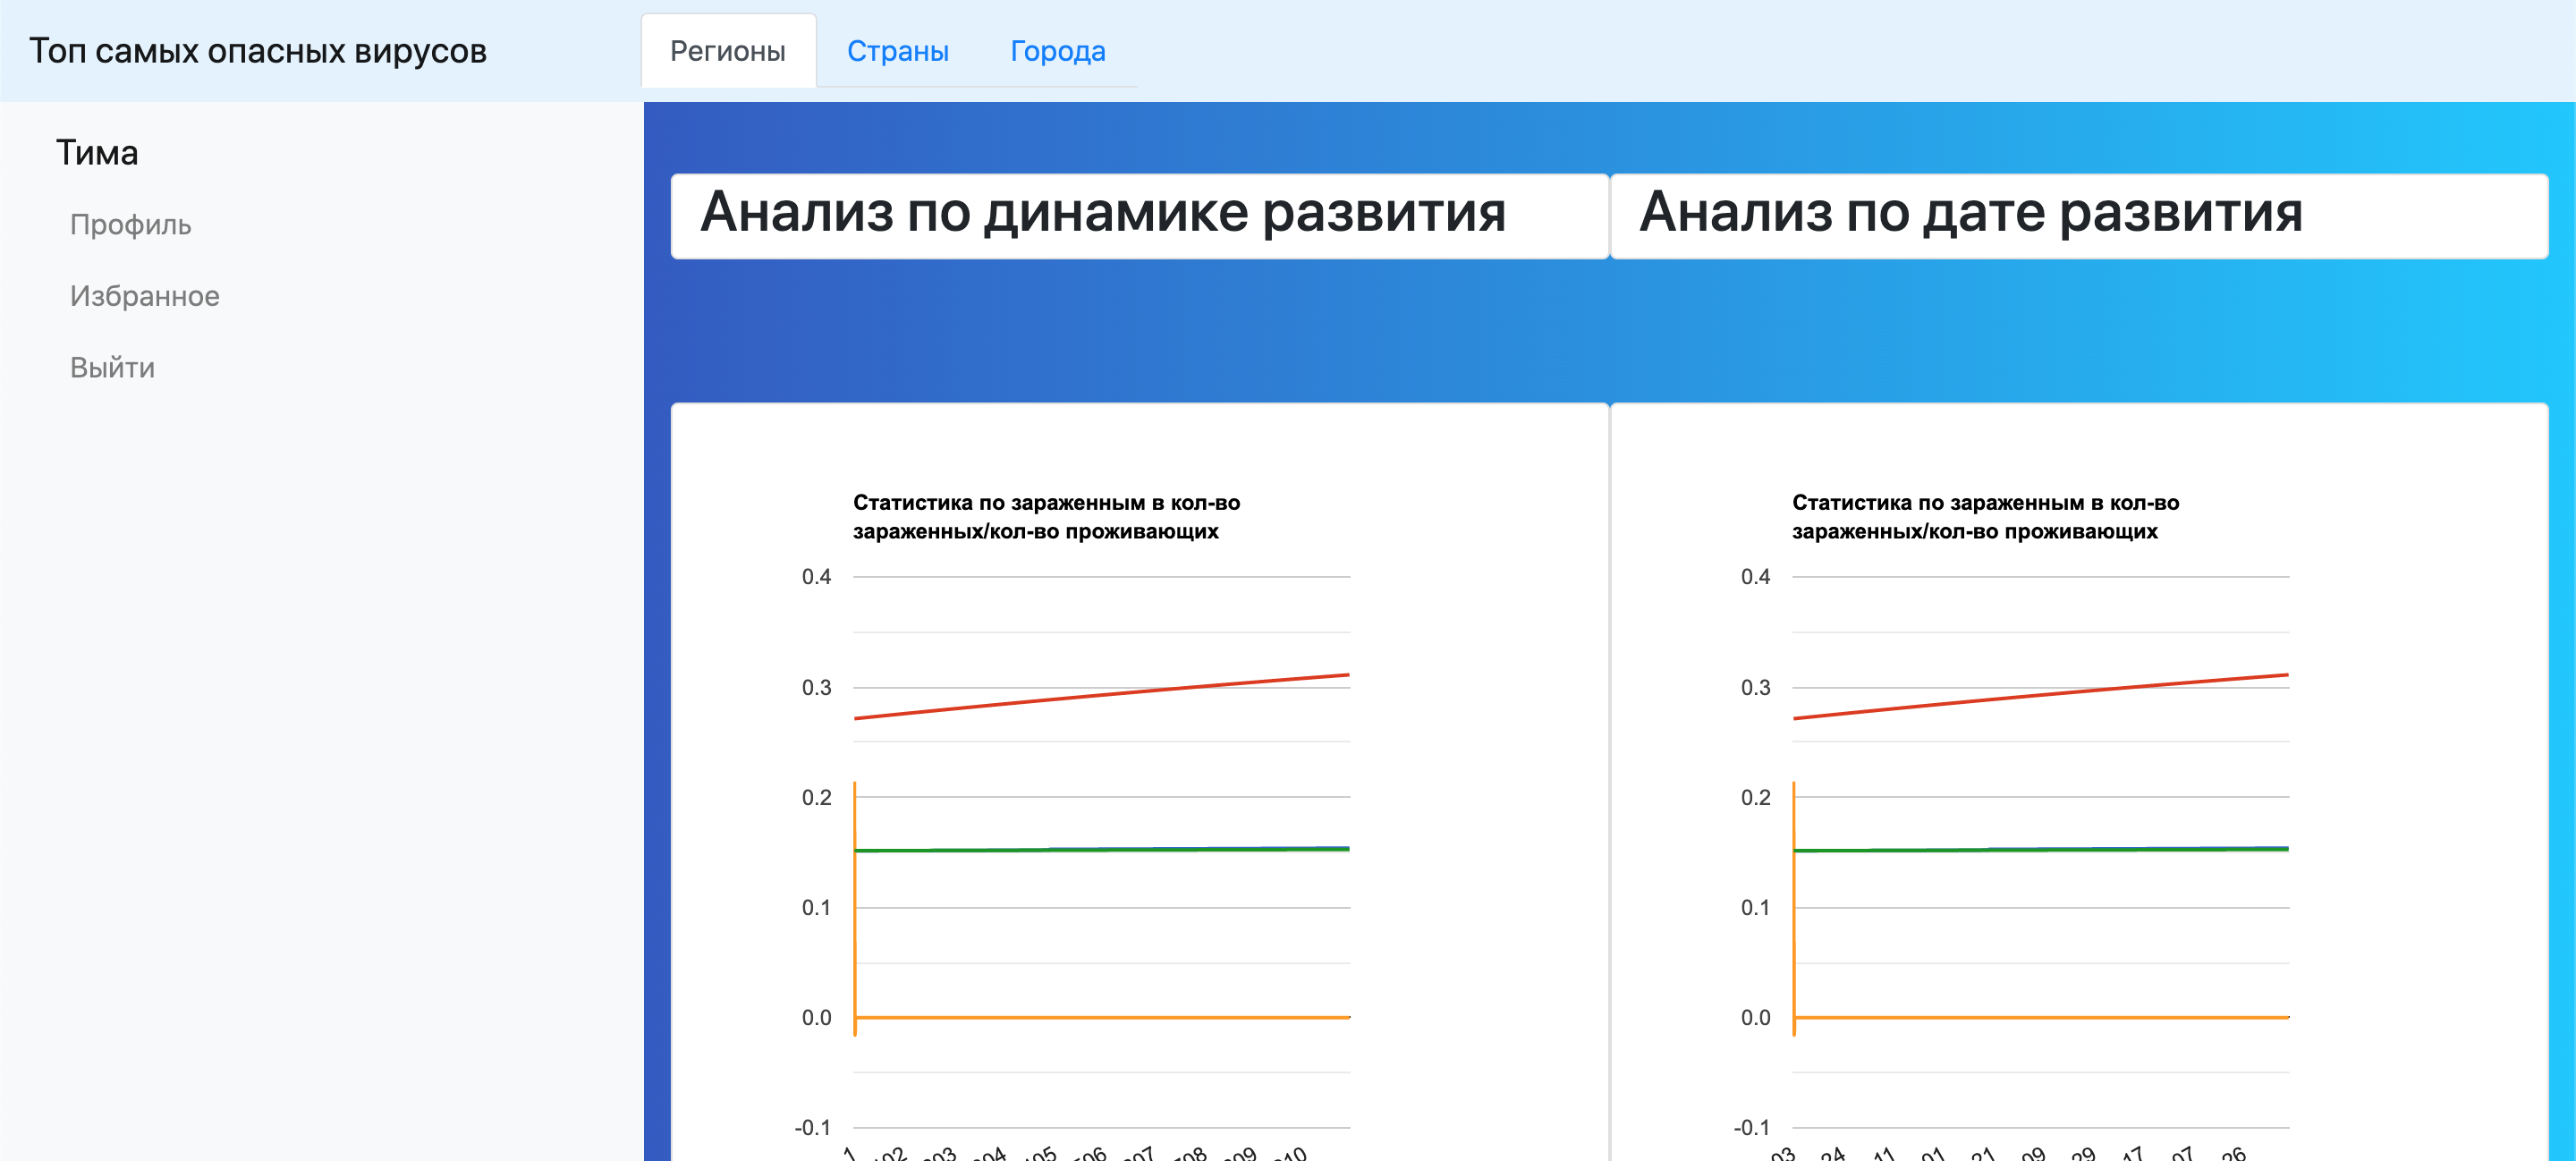
\includegraphics[width = \textwidth]{examples/graph1.png}}
 			\caption{Регионы добавленные в избранное}
 			\label{ris:graph1}
 		\end{center}
 	\end{figure}
	\newpage
 
 	
 	Кроме того, чтобы было проще редактировать информацию о тех или иных вирусах, в системе предусмотрены дополнительные возможности для особых пользователей, администраторов сайта. Так, если мы войдем в систему под логином "ilya", мы увидим, что на странице профиля пользователя надпись <<Обычный пользователь>> сменилась на <<Администратор>>.
 	
 	\begin{figure}[h!]
 		\begin{center}
 			{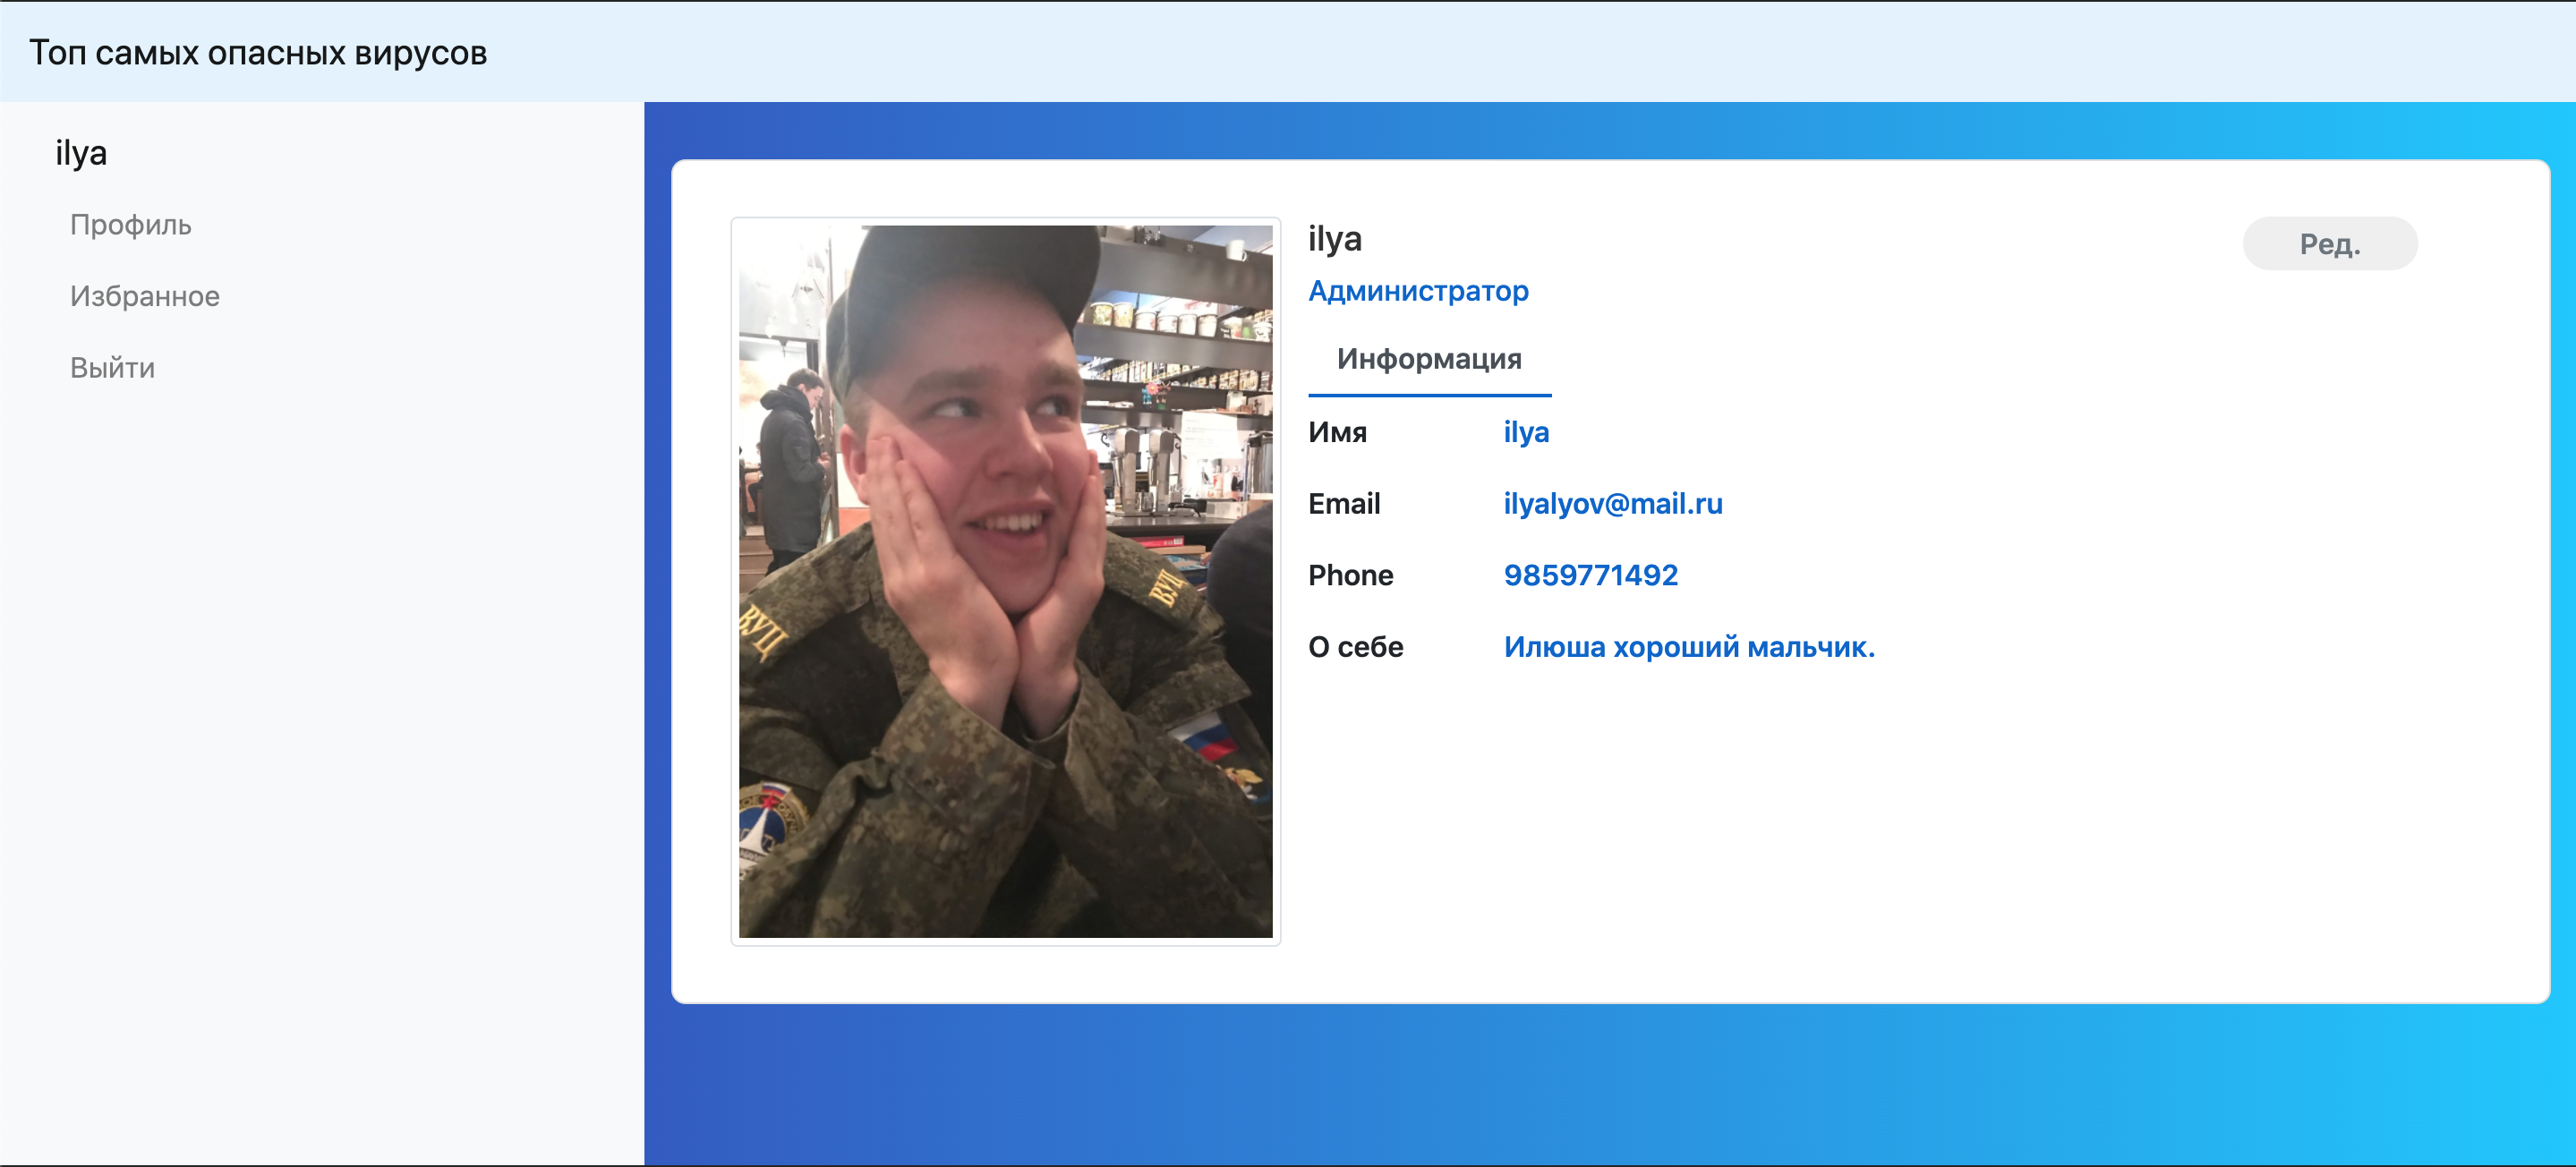
\includegraphics[width = \textwidth]{examples/profile_admin.png}}
 			\caption{
 				Главная страница (список вирусов) с возможностью добавлять элементы в избранное}
 			\label{ris:profile_admin}
 		\end{center}
 	\end{figure}
 	
 	При просмотре дополнительной информации какого-либо вируса или эпидемии появится кнопка <<Редактировать информацию>>.
 	
 	
 	\begin{figure}[h!]
 		\begin{minipage}[b]{0.45\textwidth}
 			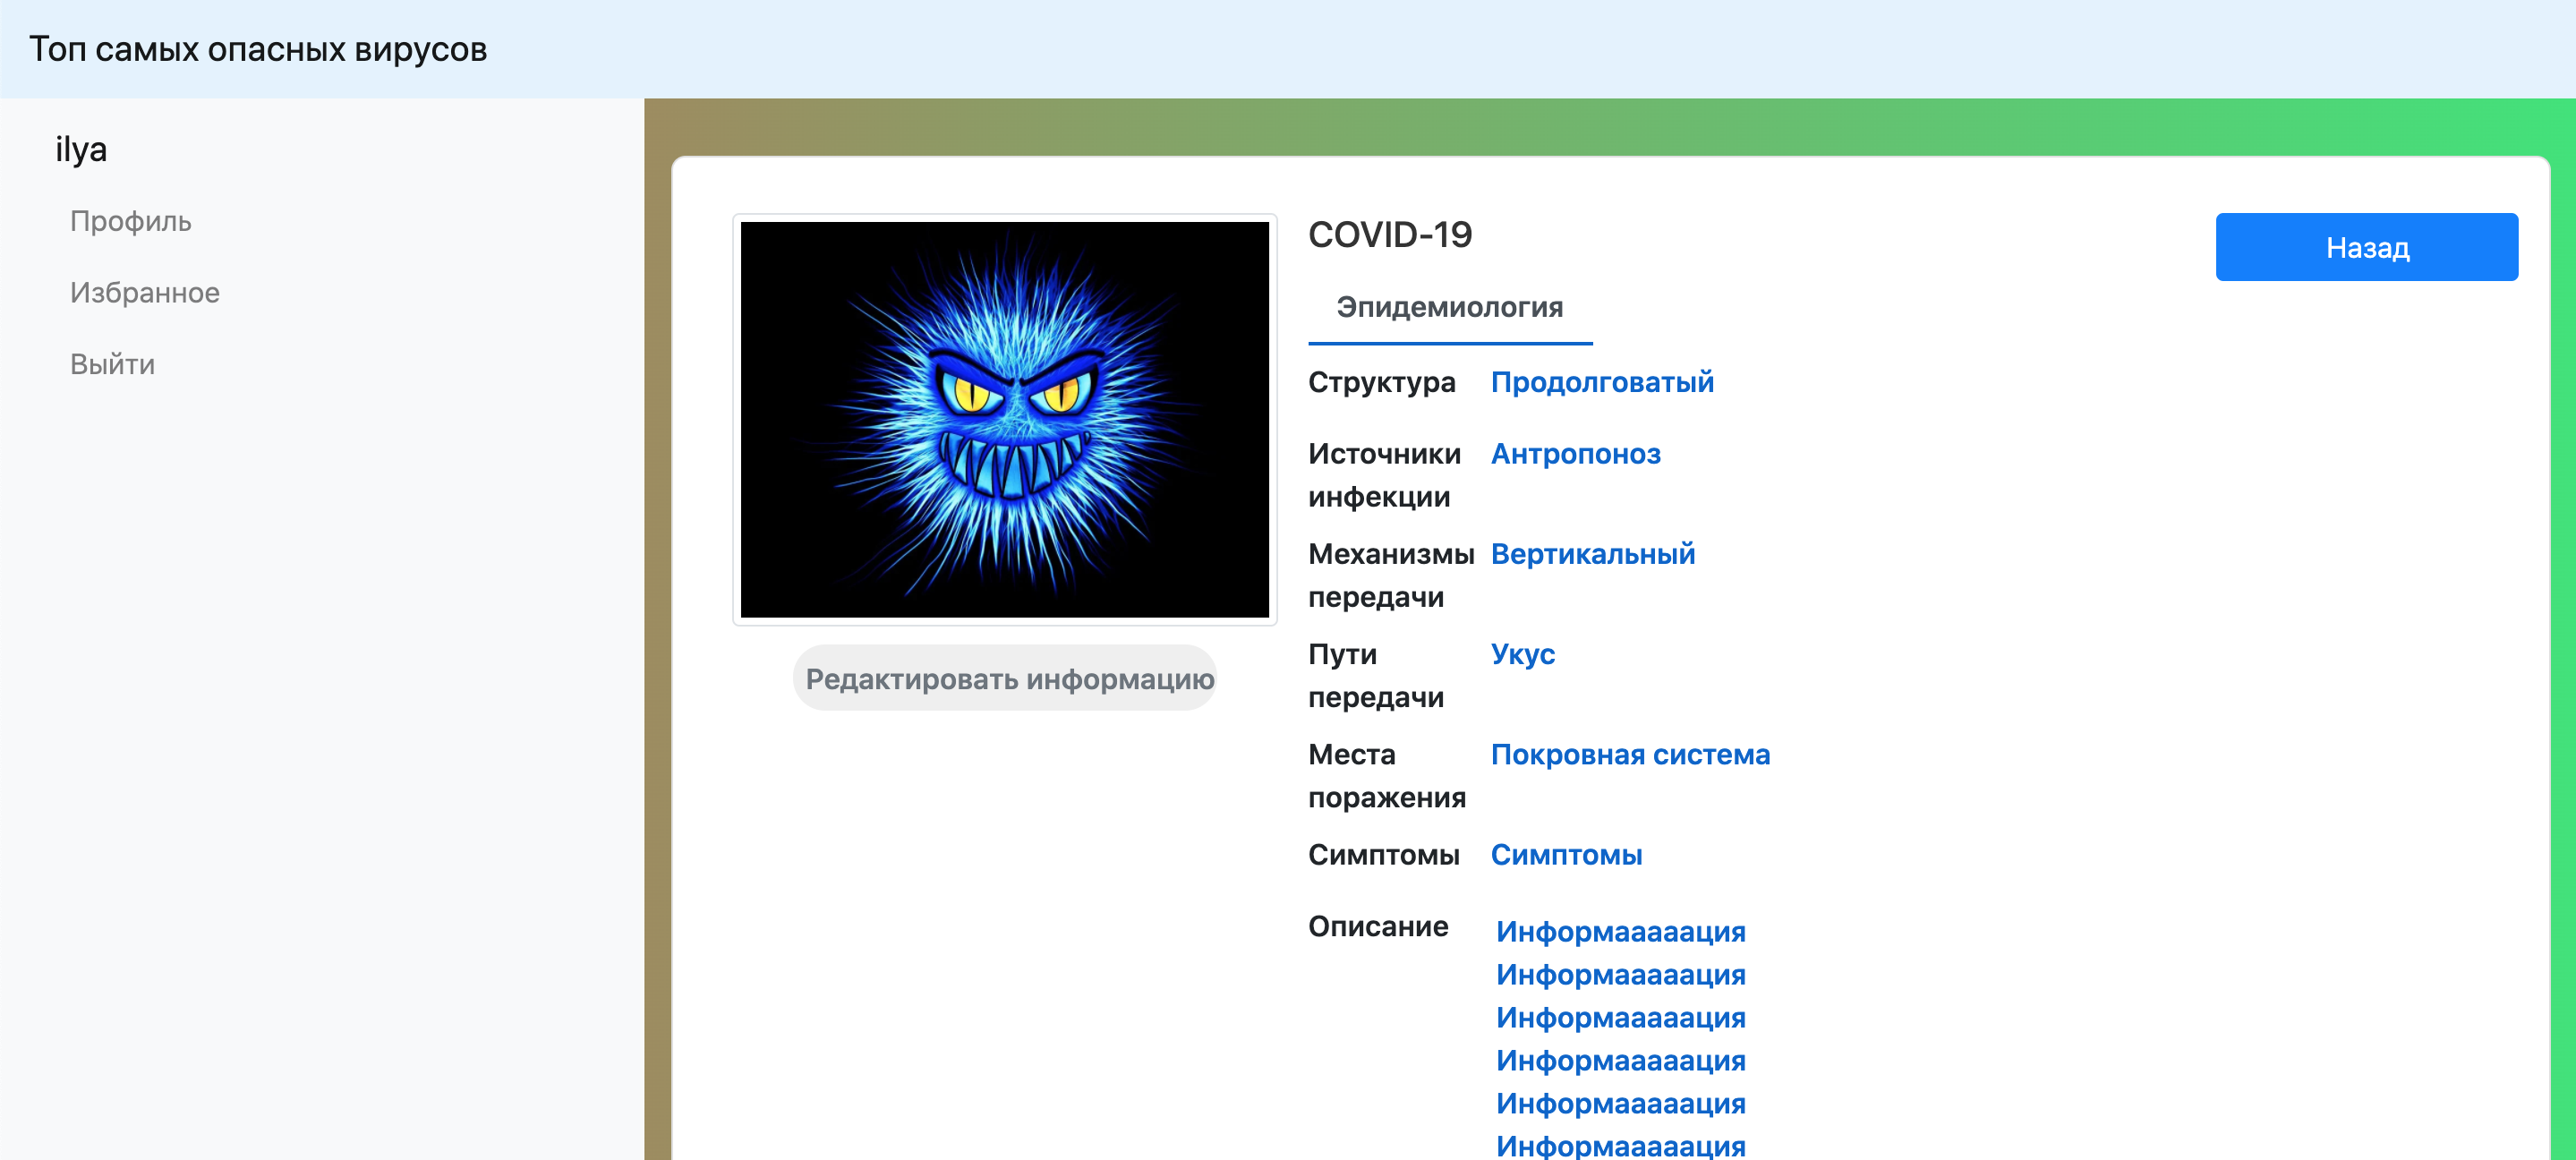
\includegraphics[width=\textwidth]{examples/more_virus_admin.png}
 			\center{Дополнительный функционал для администраторов}
 		\end{minipage}
 		\begin{minipage}[b]{0.45\textwidth}
 			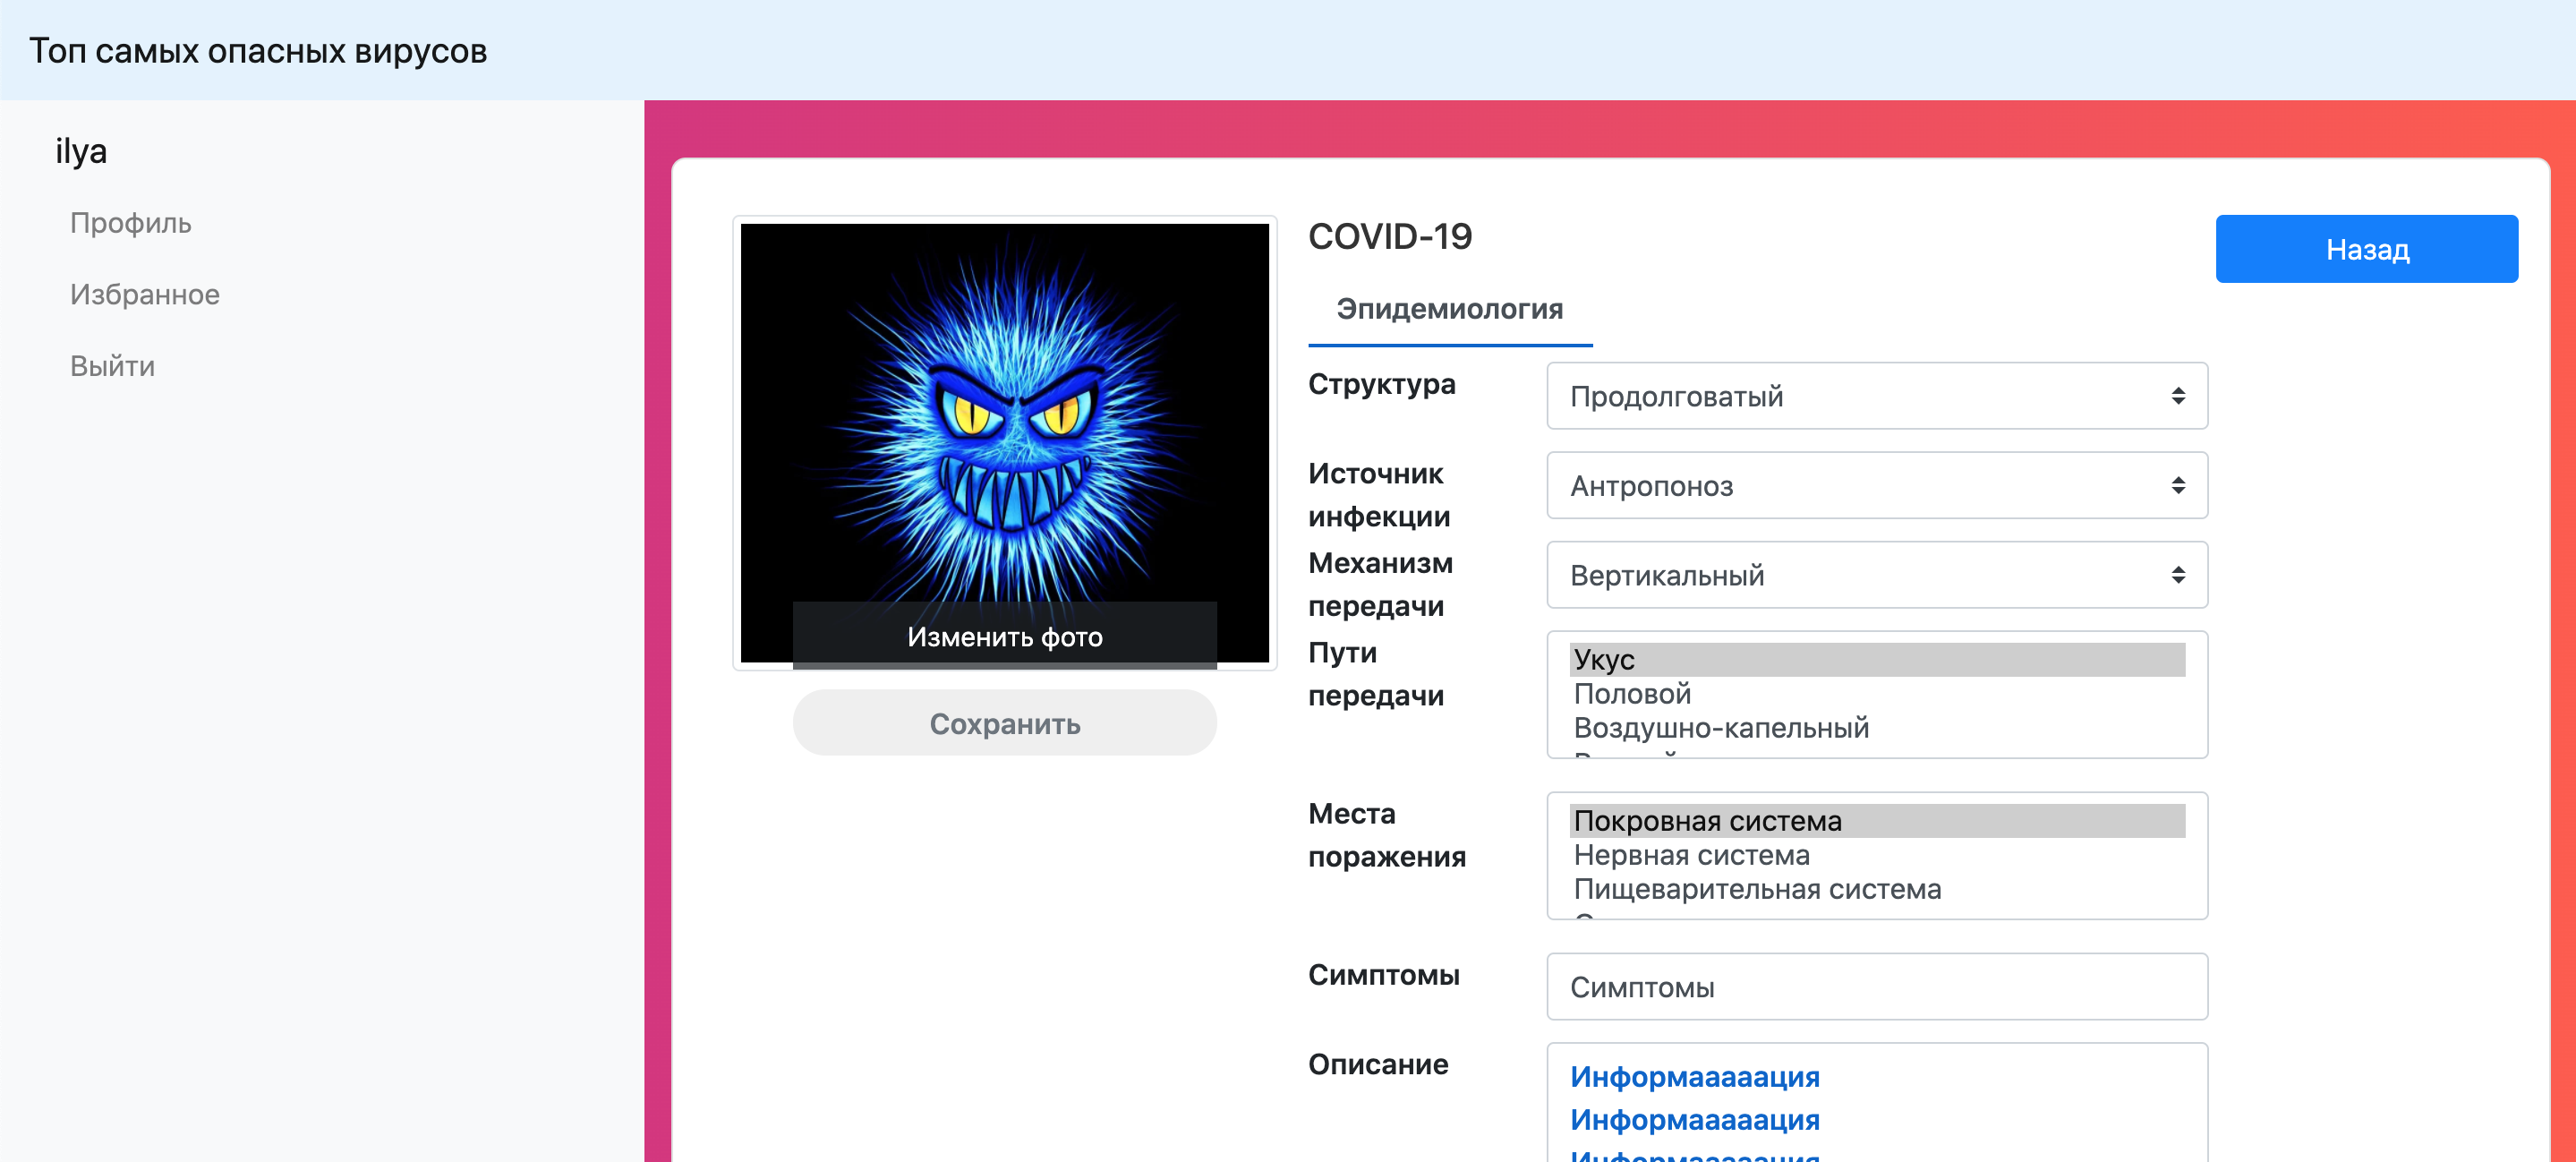
\includegraphics[width=\textwidth]{examples/edit_virus.png}
 			\center{Редактирование информации о вирусе}
 		\end{minipage}
 		\label{ris:more_virus_admin_edit_virus}
 	\end{figure}
 	
 	\newpage
 	
 	\subsection*{Выводы по технологическому разделу}
 	
 	В данном разделе были расписан основной технологический стек данной работы, были приведены реализации хранения данных, url-адресов, а также примеры реализаций контроллеров и представлений. Был описан способ заполнения базы данных.
 	
 	Также, были приведены примеры работы программы, демонстрирующие весь заявленный функционал в техническом задании.
 	
 	\newpage
 	
 	\newpage
 	\section*{Заключение}
 	\addcontentsline{toc}{section}{Заключение}
 	
 	В ходе проделанной работы был выполнен сравнительный анализ реляционных баз данных.
 	Выяснилось, что для реализации поставленной задачи
 	лучше всего подходит СУБД PostgreSQL.
 	
 	Кроме того, была спроектирована архитектура программы на основе шаблона MVC.
 	
 	В итоге, с помощью СУБД PostgreSQL и фреймворка Django было реализовано
 	веб-приложение для хранения, просмотра и анализа информации о различных вирусах. Программа подходит как для личного, так и для командного использования.
 	
 	
 	\addcontentsline{toc}{section}{Список используемой литературы}
 	\begin{thebibliography}{19}
 		\bibitem{network}
 		Основные понятия баз данных [Электронный ресурс]. – Режим доступа: 
 		http://inf.susu.ac.ru/Klinachev/lc\_sga\_26.htm, 
 		свободный – (11.07.2020)
 		
 		\bibitem{network}
 		Реляционная модель данных: теоретические основы [Электронный ресурс]. – Режим доступа: 
 		https://function-x.ru/sql\_relation\_data\_model.html, 
 		свободный – (11.07.2020)
 		
 		\bibitem{sql}
 		Джеймс Р. Грофф, Пол Н. Вайнберг, Эндрю Дж. Оппель. SQL: полное руководство – М.: Вильямс, 2014
 		
 		\bibitem{er}
 		Построение реляционной структуры из ER-модели [Электронный ресурс]. – Режим доступа: 
 		https://habr.com/ru/post/50312/, 
 		свободный – (11.07.2020)
 		
 		\bibitem{usecase}
 		UML — диаграмма вариантов использования (use case diagram) [Электронный ресурс]. – Режим доступа: 
 		https://habr.com/ru/post/47940/, 
 		свободный – (11.07.2020)
 		
 		\bibitem{postgresql}
 		PostgreSQL [Электронный ресурс]. – Режим доступа: 
 		https://www.postgresql.org/, 
 		свободный – (10.07.2020)
 		
 		\bibitem{postgresql_better}
 		Чем PostgreSQL лучше других SQL баз данных с открытым исходным кодом [Электронный ресурс]. – Режим доступа: 
 		https://habr.com/ru/post/282764/, 
 		свободный – (13.07.2020)
 		
 		\bibitem{django}
 		Django [Электронный ресурс]. – Режим доступа: 
 		https://www.djangoproject.com/, 
 		свободный – (13.07.2020)
 		
 		\bibitem{mvc_info}
 		Шаблон проектирования MVC [Электронный ресурс]. – Режим доступа: 
 		https://webformyself.com/shablon-proektirovaniya-mvc/, 
 		свободный – (12.07.2020)
 		
 		\bibitem{python}
 		Python [Электронный ресурс]. – Режим доступа: 
 		https://www.python.org/, 
 		свободный – (12.07.2020)
 		
 		\bibitem{bootstrap}
 		Bootstrap [Электронный ресурс]. – Режим доступа: 
 		https://getbootstrap.com/, 
 		свободный – (12.07.2020)
 		
 		\bibitem{js}
 		JavaScript [Электронный ресурс]. – Режим доступа: 
 		https://javascript.ru/manual, 
 		свободный – (12.07.2020)
 		
 		\bibitem{html}
 		HTML5 [Электронный ресурс]. – Режим доступа: 
 		https://developer.mozilla.org/ru/docs/HTML/HTML5, 
 		свободный – (12.07.2020)
 		
 		\bibitem{css}
 		CSS3 [Электронный ресурс]. – Режим доступа: 
 		https://developer.mozilla.org/ru/docs/Web/CSS/Reference, 
 		свободный – (12.07.2020)
 		
 		\bibitem{psycopg2}
 		Psycopg – PostgreSQL database adapter for Python [Электронный ресурс]. – Режим доступа: 
 		https://www.psycopg.org/docs/, 
 		свободный – (12.07.2020)
 		
 		\bibitem{countries}
 		Django Countries [Электронный ресурс]. – Режим доступа: 
 		https://github.com/SmileyChris/django-countries, 
 		свободный – (12.07.2020)
 		
 		\bibitem{sqlite}
 		SQLite Documentation [Электронный ресурс]. – Режим доступа: 
 		https://www.sqlite.org/docs.html, 
 		свободный – (12.07.2020)
 		
 		\bibitem{mysql}
 		MySQL Documentation [Электронный ресурс]. – Режим доступа: 
 		https://dev.mysql.com/doc/, 
 		свободный – (12.07.2020)
 		
 		\bibitem{formula}
 		Дроздюк А. Логистическая кривая.. — Торонто: Choven 2019
 	\end{thebibliography}
 	
 \end{document}
 	